\documentclass[twoside]{book}

% Packages required by doxygen
\usepackage{calc}
\usepackage{doxygen}
\usepackage{graphicx}
\usepackage[utf8]{inputenc}
\usepackage{makeidx}
\usepackage{multicol}
\usepackage{multirow}
\usepackage{textcomp}
\usepackage[table]{xcolor}

% Font selection
\usepackage[T1]{fontenc}
\usepackage{mathptmx}
\usepackage[scaled=.90]{helvet}
\usepackage{courier}
\usepackage{amssymb}
\usepackage{sectsty}
\renewcommand{\familydefault}{\sfdefault}
\allsectionsfont{%
  \fontseries{bc}\selectfont%
  \color{darkgray}%
}
\renewcommand{\DoxyLabelFont}{%
  \fontseries{bc}\selectfont%
  \color{darkgray}%
}

% Page & text layout
\usepackage{geometry}
\geometry{%
  a4paper,%
  top=2.5cm,%
  bottom=2.5cm,%
  left=2.5cm,%
  right=2.5cm%
}
\tolerance=750
\hfuzz=15pt
\hbadness=750
\setlength{\emergencystretch}{15pt}
\setlength{\parindent}{0cm}
\setlength{\parskip}{0.2cm}
\makeatletter
\renewcommand{\paragraph}{%
  \@startsection{paragraph}{4}{0ex}{-1.0ex}{1.0ex}{%
    \normalfont\normalsize\bfseries\SS@parafont%
  }%
}
\renewcommand{\subparagraph}{%
  \@startsection{subparagraph}{5}{0ex}{-1.0ex}{1.0ex}{%
    \normalfont\normalsize\bfseries\SS@subparafont%
  }%
}
\makeatother

% Headers & footers
\usepackage{fancyhdr}
\pagestyle{fancyplain}
\fancyhead[LE]{\fancyplain{}{\bfseries\thepage}}
\fancyhead[CE]{\fancyplain{}{}}
\fancyhead[RE]{\fancyplain{}{\bfseries\leftmark}}
\fancyhead[LO]{\fancyplain{}{\bfseries\rightmark}}
\fancyhead[CO]{\fancyplain{}{}}
\fancyhead[RO]{\fancyplain{}{\bfseries\thepage}}
\fancyfoot[LE]{\fancyplain{}{}}
\fancyfoot[CE]{\fancyplain{}{}}
\fancyfoot[RE]{\fancyplain{}{\bfseries\scriptsize Generated on Mon Dec 8 2014 16\-:02\-:32 for Http Server by Doxygen }}
\fancyfoot[LO]{\fancyplain{}{\bfseries\scriptsize Generated on Mon Dec 8 2014 16\-:02\-:32 for Http Server by Doxygen }}
\fancyfoot[CO]{\fancyplain{}{}}
\fancyfoot[RO]{\fancyplain{}{}}
\renewcommand{\footrulewidth}{0.4pt}
\renewcommand{\chaptermark}[1]{%
  \markboth{#1}{}%
}
\renewcommand{\sectionmark}[1]{%
  \markright{\thesection\ #1}%
}

% Indices & bibliography
\usepackage{natbib}
\usepackage[titles]{tocloft}
\setcounter{tocdepth}{3}
\setcounter{secnumdepth}{5}
\makeindex

% Hyperlinks (required, but should be loaded last)
\usepackage{ifpdf}
\ifpdf
  \usepackage[pdftex,pagebackref=true]{hyperref}
\else
  \usepackage[ps2pdf,pagebackref=true]{hyperref}
\fi
\hypersetup{%
  colorlinks=true,%
  linkcolor=blue,%
  citecolor=blue,%
  unicode%
}

% Custom commands
\newcommand{\clearemptydoublepage}{%
  \newpage{\pagestyle{empty}\cleardoublepage}%
}


%===== C O N T E N T S =====

\begin{document}

% Titlepage & ToC
\hypersetup{pageanchor=false}
\pagenumbering{roman}
\begin{titlepage}
\vspace*{7cm}
\begin{center}%
{\Large Http Server \\[1ex]\large 0.\-1 }\\
\vspace*{1cm}
{\large Generated by Doxygen 1.8.6}\\
\vspace*{0.5cm}
{\small Mon Dec 8 2014 16:02:32}\\
\end{center}
\end{titlepage}
\clearemptydoublepage
\tableofcontents
\clearemptydoublepage
\pagenumbering{arabic}
\hypersetup{pageanchor=true}

%--- Begin generated contents ---
\chapter{Namespace Index}
\section{Namespace List}
Here is a list of all documented namespaces with brief descriptions\-:\begin{DoxyCompactList}
\item\contentsline{section}{\hyperlink{namespace_connection_manager}{Connection\-Manager} \\*The \hyperlink{namespace_connection_manager}{Connection\-Manager} module contains all of the necessary classes for handling a connection }{\pageref{namespace_connection_manager}}{}
\item\contentsline{section}{\hyperlink{namespace_event_dispatcher}{Event\-Dispatcher} \\*The Event\-Dispatcher module contains classes used to implement the {\itshape Observer Pattern} }{\pageref{namespace_event_dispatcher}}{}
\end{DoxyCompactList}

\chapter{Hierarchical Index}
\section{Class Hierarchy}
This inheritance list is sorted roughly, but not completely, alphabetically\-:\begin{DoxyCompactList}
\item Event\-Dispatcher\begin{DoxyCompactList}
\item \contentsline{section}{Async\-Http\-Server.\-Async\-Http\-Server}{\pageref{class_async_http_server_1_1_async_http_server}}{}
\item \contentsline{section}{Connection\-Manager.\-Connection}{\pageref{class_connection_manager_1_1_connection}}{}
\item \contentsline{section}{Connection\-Manager.\-Connection\-Manager}{\pageref{class_connection_manager_1_1_connection_manager}}{}
\item \contentsline{section}{Http\-Request\-Handler.\-Http\-Request\-Handler}{\pageref{class_http_request_handler_1_1_http_request_handler}}{}
\item \contentsline{section}{Task\-Manager.\-Task}{\pageref{class_task_manager_1_1_task}}{}
\item \contentsline{section}{Task\-Manager.\-Task\-Manager}{\pageref{class_task_manager_1_1_task_manager}}{}
\end{DoxyCompactList}
\item object\begin{DoxyCompactList}
\item \contentsline{section}{Connection\-Manager.\-Buffer}{\pageref{class_connection_manager_1_1_buffer}}{}
\item \contentsline{section}{Event\-Dispatcher.\-Entry}{\pageref{class_event_dispatcher_1_1_entry}}{}
\item \contentsline{section}{Event\-Dispatcher.\-Event}{\pageref{class_event_dispatcher_1_1_event}}{}
\item \contentsline{section}{Event\-Dispatcher.\-Event\-Handler}{\pageref{class_event_dispatcher_1_1_event_handler}}{}
\begin{DoxyCompactList}
\item \contentsline{section}{Event\-Dispatcher.\-Event\-Dispatcher}{\pageref{class_event_dispatcher_1_1_event_dispatcher}}{}
\end{DoxyCompactList}
\item \contentsline{section}{Http\-Request.\-Http\-Request}{\pageref{class_http_request_1_1_http_request}}{}
\item \contentsline{section}{Http\-Request\-Handler.\-Http\-Request}{\pageref{class_http_request_handler_1_1_http_request}}{}
\item \contentsline{section}{Http\-Response.\-Http\-Response}{\pageref{class_http_response_1_1_http_response}}{}
\end{DoxyCompactList}
\item Thread\begin{DoxyCompactList}
\item \contentsline{section}{Task\-Manager.\-Task}{\pageref{class_task_manager_1_1_task}}{}
\end{DoxyCompactList}
\end{DoxyCompactList}

\chapter{Class Index}
\section{Class List}
Here are the classes, structs, unions and interfaces with brief descriptions\-:\begin{DoxyCompactList}
\item\contentsline{section}{\hyperlink{class_async_http_server_1_1_async_http_server}{Async\-Http\-Server.\-Async\-Http\-Server} \\*Class representing an asynchronous Http Server capable of handling G\-E\-T and P\-O\-S\-T requests }{\pageref{class_async_http_server_1_1_async_http_server}}{}
\item\contentsline{section}{\hyperlink{class_connection_manager_1_1_buffer}{Connection\-Manager.\-Buffer} \\*Class representing a byte buffer }{\pageref{class_connection_manager_1_1_buffer}}{}
\item\contentsline{section}{\hyperlink{class_connection_manager_1_1_connection}{Connection\-Manager.\-Connection} \\*Class representing a physical connection to the server }{\pageref{class_connection_manager_1_1_connection}}{}
\item\contentsline{section}{\hyperlink{class_connection_manager_1_1_connection_manager}{Connection\-Manager.\-Connection\-Manager} \\*Class used for managing active connections }{\pageref{class_connection_manager_1_1_connection_manager}}{}
\item\contentsline{section}{\hyperlink{class_event_dispatcher_1_1_entry}{Event\-Dispatcher.\-Entry} \\*Class representing a (handler, event code) pair }{\pageref{class_event_dispatcher_1_1_entry}}{}
\item\contentsline{section}{\hyperlink{class_event_dispatcher_1_1_event}{Event\-Dispatcher.\-Event} \\*Class representing an event }{\pageref{class_event_dispatcher_1_1_event}}{}
\item\contentsline{section}{\hyperlink{class_event_dispatcher_1_1_event_dispatcher}{Event\-Dispatcher.\-Event\-Dispatcher} \\*The \hyperlink{class_event_dispatcher_1_1_event_dispatcher}{Event\-Dispatcher} class is used for dispatching events }{\pageref{class_event_dispatcher_1_1_event_dispatcher}}{}
\item\contentsline{section}{\hyperlink{class_event_dispatcher_1_1_event_handler}{Event\-Dispatcher.\-Event\-Handler} \\*Abstract class for event handlers }{\pageref{class_event_dispatcher_1_1_event_handler}}{}
\item\contentsline{section}{\hyperlink{class_http_request_1_1_http_request}{Http\-Request.\-Http\-Request} \\*This class represents an Http-\/\-Request to a server }{\pageref{class_http_request_1_1_http_request}}{}
\item\contentsline{section}{\hyperlink{class_http_request_handler_1_1_http_request}{Http\-Request\-Handler.\-Http\-Request} }{\pageref{class_http_request_handler_1_1_http_request}}{}
\item\contentsline{section}{\hyperlink{class_http_request_handler_1_1_http_request_handler}{Http\-Request\-Handler.\-Http\-Request\-Handler} }{\pageref{class_http_request_handler_1_1_http_request_handler}}{}
\item\contentsline{section}{\hyperlink{class_http_response_1_1_http_response}{Http\-Response.\-Http\-Response} }{\pageref{class_http_response_1_1_http_response}}{}
\item\contentsline{section}{\hyperlink{class_task_manager_1_1_task}{Task\-Manager.\-Task} }{\pageref{class_task_manager_1_1_task}}{}
\item\contentsline{section}{\hyperlink{class_task_manager_1_1_task_manager}{Task\-Manager.\-Task\-Manager} }{\pageref{class_task_manager_1_1_task_manager}}{}
\end{DoxyCompactList}

\chapter{Namespace Documentation}
\hypertarget{namespace_connection_manager}{\section{Connection\-Manager Namespace Reference}
\label{namespace_connection_manager}\index{Connection\-Manager@{Connection\-Manager}}
}


The \hyperlink{namespace_connection_manager}{Connection\-Manager} module contains all of the necessary classes for handling a connection.  


\subsection*{Classes}
\begin{DoxyCompactItemize}
\item 
class \hyperlink{class_connection_manager_1_1_buffer}{Buffer}
\begin{DoxyCompactList}\small\item\em Class representing a byte buffer. \end{DoxyCompactList}\item 
class \hyperlink{class_connection_manager_1_1_connection}{Connection}
\begin{DoxyCompactList}\small\item\em Class representing a physical connection to the server. \end{DoxyCompactList}\item 
class \hyperlink{class_connection_manager_1_1_connection_manager}{Connection\-Manager}
\begin{DoxyCompactList}\small\item\em Class used for managing active connections. \end{DoxyCompactList}\end{DoxyCompactItemize}
\subsection*{Variables}
\begin{DoxyCompactItemize}
\item 
\hypertarget{namespace_connection_manager_acf0b032340426584ea50a6ce0ac79f84}{string {\bfseries \-\_\-\-\_\-author\-\_\-\-\_\-} = 'Ivan Dortulov'}\label{namespace_connection_manager_acf0b032340426584ea50a6ce0ac79f84}

\end{DoxyCompactItemize}


\subsection{Detailed Description}
The \hyperlink{namespace_connection_manager}{Connection\-Manager} module contains all of the necessary classes for handling a connection. It consists of two classes\-: \hyperlink{class_connection_manager_1_1_connection}{Connection} and \hyperlink{namespace_connection_manager}{Connection\-Manager}.

The \hyperlink{class_connection_manager_1_1_connection}{Connection} class is just a simple representation of a connection. It contains a socket handle used to send and receive data, an input\-\_\-buffer which stores the data received from the socket and an output\-\_\-buffer from which data is sent to the socket.

The \hyperlink{namespace_connection_manager}{Connection\-Manager} class creates the \hyperlink{class_connection_manager_1_1_connection}{Connection} objects. It receives messages from the Web\-Server class informing it when new connections have been established and when data has been received. It is responsible for managing the \hyperlink{class_connection_manager_1_1_connection}{Connection} objects. 
\hypertarget{namespace_event_dispatcher}{\section{Event\-Dispatcher Namespace Reference}
\label{namespace_event_dispatcher}\index{Event\-Dispatcher@{Event\-Dispatcher}}
}


The Event\-Dispatcher module contains classes used to implement the {\itshape Observer Pattern}.  


\subsection*{Classes}
\begin{DoxyCompactItemize}
\item 
class \hyperlink{class_event_dispatcher_1_1_entry}{Entry}
\begin{DoxyCompactList}\small\item\em Class representing a (handler, event code) pair. \end{DoxyCompactList}\item 
class \hyperlink{class_event_dispatcher_1_1_event}{Event}
\begin{DoxyCompactList}\small\item\em Class representing an event. \end{DoxyCompactList}\item 
class \hyperlink{class_event_dispatcher_1_1_event_handler}{Event\-Handler}
\begin{DoxyCompactList}\small\item\em Abstract class for event handlers. \end{DoxyCompactList}\item 
class \hyperlink{class_event_dispatcher_1_1_event_dispatcher}{Event\-Dispatcher}
\begin{DoxyCompactList}\small\item\em The \hyperlink{class_event_dispatcher_1_1_event_dispatcher}{Event\-Dispatcher} class is used for dispatching events. \end{DoxyCompactList}\end{DoxyCompactItemize}
\subsection*{Variables}
\begin{DoxyCompactItemize}
\item 
\hypertarget{namespace_event_dispatcher_aebf383ab1c47c4d3f05a6bb89e660f3e}{string {\bfseries \-\_\-\-\_\-author\-\_\-\-\_\-} = 'Ivan Dortulov'}\label{namespace_event_dispatcher_aebf383ab1c47c4d3f05a6bb89e660f3e}

\end{DoxyCompactItemize}


\subsection{Detailed Description}
The Event\-Dispatcher module contains classes used to implement the {\itshape Observer Pattern}. It consists of three main components \hyperlink{class_event_dispatcher_1_1_event}{Event}, \hyperlink{class_event_dispatcher_1_1_event_handler}{Event\-Handler} and Event\-Dispatcher.

Events can be anything inside your application from a user clicking a button, a file being opened, a socket being closed to a thread finishing its execution. It is used for communication between the components of the Async\-Server.

The \hyperlink{class_event_dispatcher_1_1_event_handler}{Event\-Handler} is an abstract class containing only one method called handle\-\_\-event(). Each \hyperlink{class_event_dispatcher_1_1_event_handler}{Event\-Handler} is associated with a given event code. When the event occurs the handle\-\_\-event() method of the appropriate \hyperlink{class_event_dispatcher_1_1_event_handler}{Event\-Handler} is called to handle that event.

The Event\-Dispatcher class is used to dispatch messages to the \hyperlink{class_event_dispatcher_1_1_event_handler}{Event\-Handler}. 
\chapter{Class Documentation}
\hypertarget{class_async_http_server_1_1_async_http_server}{\section{Async\-Http\-Server.\-Async\-Http\-Server Class Reference}
\label{class_async_http_server_1_1_async_http_server}\index{Async\-Http\-Server.\-Async\-Http\-Server@{Async\-Http\-Server.\-Async\-Http\-Server}}
}


Class representing an asynchronous Http Server capable of handling G\-E\-T and P\-O\-S\-T requests.  


Inheritance diagram for Async\-Http\-Server.\-Async\-Http\-Server\-:\begin{figure}[H]
\begin{center}
\leavevmode
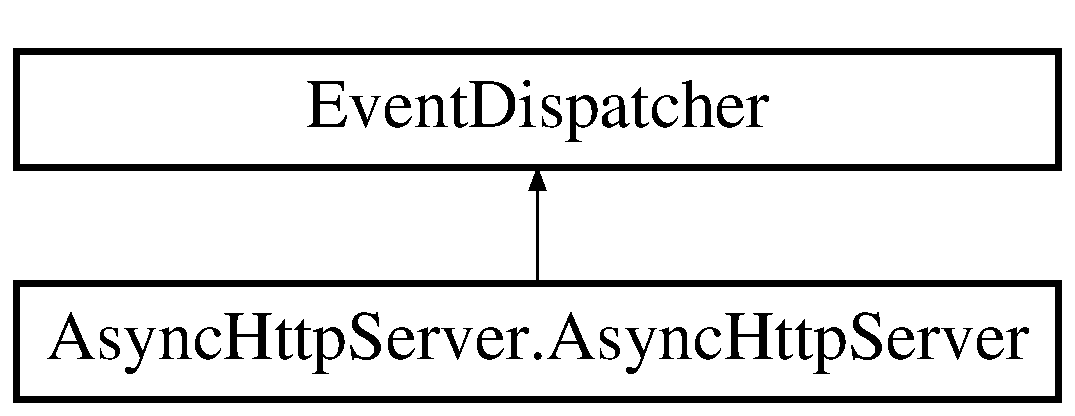
\includegraphics[height=2.000000cm]{class_async_http_server_1_1_async_http_server}
\end{center}
\end{figure}
\subsection*{Public Member Functions}
\begin{DoxyCompactItemize}
\item 
\hypertarget{class_async_http_server_1_1_async_http_server_a1f40cb27ad3596f0cfe7d485d4915a60}{def \hyperlink{class_async_http_server_1_1_async_http_server_a1f40cb27ad3596f0cfe7d485d4915a60}{\-\_\-\-\_\-init\-\_\-\-\_\-}}\label{class_async_http_server_1_1_async_http_server_a1f40cb27ad3596f0cfe7d485d4915a60}

\begin{DoxyCompactList}\small\item\em Default constructor. \end{DoxyCompactList}\item 
\hypertarget{class_async_http_server_1_1_async_http_server_a6bdeabbfb533d9ab41a775e1e7bd56c4}{def \hyperlink{class_async_http_server_1_1_async_http_server_a6bdeabbfb533d9ab41a775e1e7bd56c4}{server\-\_\-bind}}\label{class_async_http_server_1_1_async_http_server_a6bdeabbfb533d9ab41a775e1e7bd56c4}

\begin{DoxyCompactList}\small\item\em Bind the server socket. \end{DoxyCompactList}\item 
def \hyperlink{class_async_http_server_1_1_async_http_server_ac30900bc1acbf9ed8c97f09874ca6140}{server\-\_\-activate}
\begin{DoxyCompactList}\small\item\em Activate the server. \end{DoxyCompactList}\item 
def \hyperlink{class_async_http_server_1_1_async_http_server_a2e97316d792b48283feeb9ae1e7427e6}{server\-\_\-forever}
\begin{DoxyCompactList}\small\item\em Start the server. \end{DoxyCompactList}\end{DoxyCompactItemize}
\subsection*{Public Attributes}
\begin{DoxyCompactItemize}
\item 
\hypertarget{class_async_http_server_1_1_async_http_server_a9e643118346eb938e71094a6867f40e3}{\hyperlink{class_async_http_server_1_1_async_http_server_a9e643118346eb938e71094a6867f40e3}{running}}\label{class_async_http_server_1_1_async_http_server_a9e643118346eb938e71094a6867f40e3}

\begin{DoxyCompactList}\small\item\em Is the server currently running. \end{DoxyCompactList}\item 
\hypertarget{class_async_http_server_1_1_async_http_server_a84fd8d5d5ab2a0ef2ceaf3fbf29e194a}{\hyperlink{class_async_http_server_1_1_async_http_server_a84fd8d5d5ab2a0ef2ceaf3fbf29e194a}{server\-\_\-address}}\label{class_async_http_server_1_1_async_http_server_a84fd8d5d5ab2a0ef2ceaf3fbf29e194a}

\begin{DoxyCompactList}\small\item\em The host address of the server. \end{DoxyCompactList}\item 
\hypertarget{class_async_http_server_1_1_async_http_server_abac435708c22ad21af620e3a704d4bfd}{\hyperlink{class_async_http_server_1_1_async_http_server_abac435708c22ad21af620e3a704d4bfd}{server\-\_\-port}}\label{class_async_http_server_1_1_async_http_server_abac435708c22ad21af620e3a704d4bfd}

\begin{DoxyCompactList}\small\item\em The port on which the server is listening for incoming connections. \end{DoxyCompactList}\item 
\hyperlink{class_async_http_server_1_1_async_http_server_aab2a41d288f15308d305bff00e922200}{connection\-\_\-manager}
\begin{DoxyCompactList}\small\item\em Instance of the \hyperlink{namespace_connection_manager}{Connection\-Manager} class. \end{DoxyCompactList}\item 
\hyperlink{class_async_http_server_1_1_async_http_server_ad6c600941d9ab1f0e5880290db2dcb93}{address\-\_\-family}
\begin{DoxyCompactList}\small\item\em The address family of the server. \end{DoxyCompactList}\item 
\hyperlink{class_async_http_server_1_1_async_http_server_ae703825864891b7c4f1f69eb541eb64f}{socket\-\_\-type}
\begin{DoxyCompactList}\small\item\em The type of the socket. \end{DoxyCompactList}\item 
\hypertarget{class_async_http_server_1_1_async_http_server_a8ce24f83f3acafe8756d1ba1ade13752}{\hyperlink{class_async_http_server_1_1_async_http_server_a8ce24f83f3acafe8756d1ba1ade13752}{socket}}\label{class_async_http_server_1_1_async_http_server_a8ce24f83f3acafe8756d1ba1ade13752}

\begin{DoxyCompactList}\small\item\em The server socket used for listening. \end{DoxyCompactList}\end{DoxyCompactItemize}


\subsection{Detailed Description}
Class representing an asynchronous Http Server capable of handling G\-E\-T and P\-O\-S\-T requests. 

The server uses an asynchronous approach to handle the incoming request. Each time a client connects, that client's socket gets associated with a Connection object.\par
 The Connection object uses the Http\-Request\-Handler class (each Connection object instantiates Http\-Request\-Handler) to process incoming request.\par
 Whenever a resource is request the Http\-Response\-Handler tells the Task\-Manager class to create a new Task for obtaining the file. 

\subsection{Member Function Documentation}
\hypertarget{class_async_http_server_1_1_async_http_server_ac30900bc1acbf9ed8c97f09874ca6140}{\index{Async\-Http\-Server\-::\-Async\-Http\-Server@{Async\-Http\-Server\-::\-Async\-Http\-Server}!server\-\_\-activate@{server\-\_\-activate}}
\index{server\-\_\-activate@{server\-\_\-activate}!AsyncHttpServer::AsyncHttpServer@{Async\-Http\-Server\-::\-Async\-Http\-Server}}
\subsubsection[{server\-\_\-activate}]{\setlength{\rightskip}{0pt plus 5cm}def Async\-Http\-Server.\-Async\-Http\-Server.\-server\-\_\-activate (
\begin{DoxyParamCaption}
\item[{}]{self}
\end{DoxyParamCaption}
)}}\label{class_async_http_server_1_1_async_http_server_ac30900bc1acbf9ed8c97f09874ca6140}


Activate the server. 

This method calls the server socket's listen() method. \hypertarget{class_async_http_server_1_1_async_http_server_a2e97316d792b48283feeb9ae1e7427e6}{\index{Async\-Http\-Server\-::\-Async\-Http\-Server@{Async\-Http\-Server\-::\-Async\-Http\-Server}!server\-\_\-forever@{server\-\_\-forever}}
\index{server\-\_\-forever@{server\-\_\-forever}!AsyncHttpServer::AsyncHttpServer@{Async\-Http\-Server\-::\-Async\-Http\-Server}}
\subsubsection[{server\-\_\-forever}]{\setlength{\rightskip}{0pt plus 5cm}def Async\-Http\-Server.\-Async\-Http\-Server.\-server\-\_\-forever (
\begin{DoxyParamCaption}
\item[{}]{self}
\end{DoxyParamCaption}
)}}\label{class_async_http_server_1_1_async_http_server_a2e97316d792b48283feeb9ae1e7427e6}


Start the server. 

This method larches the server and makes it listen for incoming connections as well as process incoming event. 

\subsection{Member Data Documentation}
\hypertarget{class_async_http_server_1_1_async_http_server_ad6c600941d9ab1f0e5880290db2dcb93}{\index{Async\-Http\-Server\-::\-Async\-Http\-Server@{Async\-Http\-Server\-::\-Async\-Http\-Server}!address\-\_\-family@{address\-\_\-family}}
\index{address\-\_\-family@{address\-\_\-family}!AsyncHttpServer::AsyncHttpServer@{Async\-Http\-Server\-::\-Async\-Http\-Server}}
\subsubsection[{address\-\_\-family}]{\setlength{\rightskip}{0pt plus 5cm}Async\-Http\-Server.\-Async\-Http\-Server.\-address\-\_\-family}}\label{class_async_http_server_1_1_async_http_server_ad6c600941d9ab1f0e5880290db2dcb93}


The address family of the server. 

Use this variable to change the type of the server's transport protocol to T\-C\-P or U\-D\-P. Default is T\-C\-P (A\-F\-\_\-\-I\-N\-E\-T). \hypertarget{class_async_http_server_1_1_async_http_server_aab2a41d288f15308d305bff00e922200}{\index{Async\-Http\-Server\-::\-Async\-Http\-Server@{Async\-Http\-Server\-::\-Async\-Http\-Server}!connection\-\_\-manager@{connection\-\_\-manager}}
\index{connection\-\_\-manager@{connection\-\_\-manager}!AsyncHttpServer::AsyncHttpServer@{Async\-Http\-Server\-::\-Async\-Http\-Server}}
\subsubsection[{connection\-\_\-manager}]{\setlength{\rightskip}{0pt plus 5cm}Async\-Http\-Server.\-Async\-Http\-Server.\-connection\-\_\-manager}}\label{class_async_http_server_1_1_async_http_server_aab2a41d288f15308d305bff00e922200}


Instance of the \hyperlink{namespace_connection_manager}{Connection\-Manager} class. 

Only one such instance exists per server. \hypertarget{class_async_http_server_1_1_async_http_server_ae703825864891b7c4f1f69eb541eb64f}{\index{Async\-Http\-Server\-::\-Async\-Http\-Server@{Async\-Http\-Server\-::\-Async\-Http\-Server}!socket\-\_\-type@{socket\-\_\-type}}
\index{socket\-\_\-type@{socket\-\_\-type}!AsyncHttpServer::AsyncHttpServer@{Async\-Http\-Server\-::\-Async\-Http\-Server}}
\subsubsection[{socket\-\_\-type}]{\setlength{\rightskip}{0pt plus 5cm}Async\-Http\-Server.\-Async\-Http\-Server.\-socket\-\_\-type}}\label{class_async_http_server_1_1_async_http_server_ae703825864891b7c4f1f69eb541eb64f}


The type of the socket. 

Default is streaming socket (S\-O\-C\-K\-\_\-\-S\-T\-R\-E\-A\-M) 

The documentation for this class was generated from the following file\-:\begin{DoxyCompactItemize}
\item 
/home/ivan/\-Code\-Snippets-\/\-Projects/\-Telebid-\/\-Tasks/\-Web\-Server/\-Async\-Server/Async\-Http\-Server.\-py\end{DoxyCompactItemize}

\hypertarget{class_connection_manager_1_1_buffer}{\section{Connection\-Manager.\-Buffer Class Reference}
\label{class_connection_manager_1_1_buffer}\index{Connection\-Manager.\-Buffer@{Connection\-Manager.\-Buffer}}
}


Class representing a byte buffer.  


Inheritance diagram for Connection\-Manager.\-Buffer\-:\begin{figure}[H]
\begin{center}
\leavevmode
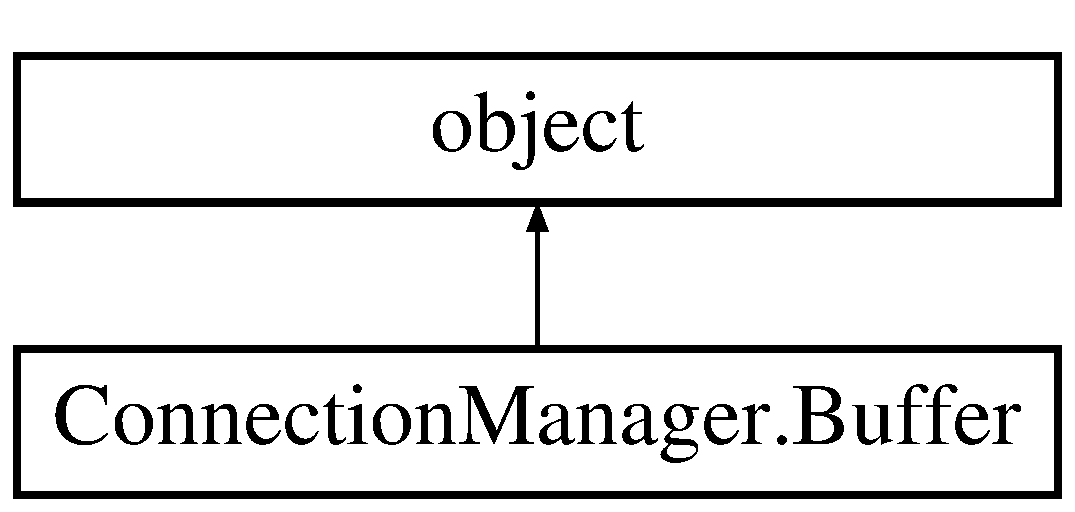
\includegraphics[height=2.000000cm]{class_connection_manager_1_1_buffer}
\end{center}
\end{figure}
\subsection*{Public Member Functions}
\begin{DoxyCompactItemize}
\item 
def \hyperlink{class_connection_manager_1_1_buffer_ab23788175bcdf08a9e4f0c2c50c6ae25}{\-\_\-\-\_\-init\-\_\-\-\_\-}
\begin{DoxyCompactList}\small\item\em Default constructor. \end{DoxyCompactList}\item 
\hypertarget{class_connection_manager_1_1_buffer_a69798f2abe4f724882166a213c1479a6}{def \hyperlink{class_connection_manager_1_1_buffer_a69798f2abe4f724882166a213c1479a6}{write}}\label{class_connection_manager_1_1_buffer_a69798f2abe4f724882166a213c1479a6}

\begin{DoxyCompactList}\small\item\em Write data to the buffer. \end{DoxyCompactList}\item 
def \hyperlink{class_connection_manager_1_1_buffer_a4d5008eacce719e83798bfa23b7212b0}{read\-\_\-line}
\begin{DoxyCompactList}\small\item\em Read a single line from the buffer. \end{DoxyCompactList}\item 
def \hyperlink{class_connection_manager_1_1_buffer_ab99c940b49904019829273977e496e8a}{get\-\_\-lines}
\begin{DoxyCompactList}\small\item\em Obtain an array of lines. \end{DoxyCompactList}\item 
def \hyperlink{class_connection_manager_1_1_buffer_a27c0a434a0faa3994e7a215f37f5409f}{to\-\_\-string}
\begin{DoxyCompactList}\small\item\em Converts the buffer to a string. \end{DoxyCompactList}\item 
def \hyperlink{class_connection_manager_1_1_buffer_a8e7aa8daa70e06dbe7e7f3156bd198ce}{empty}
\begin{DoxyCompactList}\small\item\em Checks to see if the buffer is not empty. \end{DoxyCompactList}\item 
\hypertarget{class_connection_manager_1_1_buffer_afad92674c4836d90b663d6dd364bd026}{def \hyperlink{class_connection_manager_1_1_buffer_afad92674c4836d90b663d6dd364bd026}{clear}}\label{class_connection_manager_1_1_buffer_afad92674c4836d90b663d6dd364bd026}

\begin{DoxyCompactList}\small\item\em Clear the buffer by emptying its contents. \end{DoxyCompactList}\item 
def \hyperlink{class_connection_manager_1_1_buffer_ae3d52408d0580093d8e7fdcb33a08d73}{length}
\begin{DoxyCompactList}\small\item\em Returns the number of bytes inside the buffer. \end{DoxyCompactList}\item 
def \hyperlink{class_connection_manager_1_1_buffer_a19dfa227ce76299c4b322be6c2fc6673}{find}
\begin{DoxyCompactList}\small\item\em Search the buffer for a substring. \end{DoxyCompactList}\item 
def \hyperlink{class_connection_manager_1_1_buffer_a08de35576de23a84dcd331a5154650bf}{read}
\begin{DoxyCompactList}\small\item\em Read a given number of bytes from the buffer by removing the read bytes from the buffer. \end{DoxyCompactList}\end{DoxyCompactItemize}
\subsection*{Public Attributes}
\begin{DoxyCompactItemize}
\item 
\hypertarget{class_connection_manager_1_1_buffer_a1aa7279467377362cd54f3041e6df72e}{{\bfseries buffer}}\label{class_connection_manager_1_1_buffer_a1aa7279467377362cd54f3041e6df72e}

\end{DoxyCompactItemize}


\subsection{Detailed Description}
Class representing a byte buffer. 

It is used primarily to pass data between the Http\-Request\-Handler and the \hyperlink{class_connection_manager_1_1_connection}{Connection} classes 

\subsection{Constructor \& Destructor Documentation}
\hypertarget{class_connection_manager_1_1_buffer_ab23788175bcdf08a9e4f0c2c50c6ae25}{\index{Connection\-Manager\-::\-Buffer@{Connection\-Manager\-::\-Buffer}!\-\_\-\-\_\-init\-\_\-\-\_\-@{\-\_\-\-\_\-init\-\_\-\-\_\-}}
\index{\-\_\-\-\_\-init\-\_\-\-\_\-@{\-\_\-\-\_\-init\-\_\-\-\_\-}!ConnectionManager::Buffer@{Connection\-Manager\-::\-Buffer}}
\subsubsection[{\-\_\-\-\_\-init\-\_\-\-\_\-}]{\setlength{\rightskip}{0pt plus 5cm}def Connection\-Manager.\-Buffer.\-\_\-\-\_\-init\-\_\-\-\_\- (
\begin{DoxyParamCaption}
\item[{}]{self}
\end{DoxyParamCaption}
)}}\label{class_connection_manager_1_1_buffer_ab23788175bcdf08a9e4f0c2c50c6ae25}


Default constructor. 

Constructs an empty buffer. 

\subsection{Member Function Documentation}
\hypertarget{class_connection_manager_1_1_buffer_a8e7aa8daa70e06dbe7e7f3156bd198ce}{\index{Connection\-Manager\-::\-Buffer@{Connection\-Manager\-::\-Buffer}!empty@{empty}}
\index{empty@{empty}!ConnectionManager::Buffer@{Connection\-Manager\-::\-Buffer}}
\subsubsection[{empty}]{\setlength{\rightskip}{0pt plus 5cm}def Connection\-Manager.\-Buffer.\-empty (
\begin{DoxyParamCaption}
\item[{}]{self}
\end{DoxyParamCaption}
)}}\label{class_connection_manager_1_1_buffer_a8e7aa8daa70e06dbe7e7f3156bd198ce}


Checks to see if the buffer is not empty. 

\begin{DoxyReturn}{Returns}
Returns True if the buffer is empty and False otherwise. 
\end{DoxyReturn}
\hypertarget{class_connection_manager_1_1_buffer_a19dfa227ce76299c4b322be6c2fc6673}{\index{Connection\-Manager\-::\-Buffer@{Connection\-Manager\-::\-Buffer}!find@{find}}
\index{find@{find}!ConnectionManager::Buffer@{Connection\-Manager\-::\-Buffer}}
\subsubsection[{find}]{\setlength{\rightskip}{0pt plus 5cm}def Connection\-Manager.\-Buffer.\-find (
\begin{DoxyParamCaption}
\item[{}]{self, }
\item[{}]{needle}
\end{DoxyParamCaption}
)}}\label{class_connection_manager_1_1_buffer_a19dfa227ce76299c4b322be6c2fc6673}


Search the buffer for a substring. 


\begin{DoxyParams}{Parameters}
{\em needle} & The substring to search for. \\
\hline
\end{DoxyParams}
\hypertarget{class_connection_manager_1_1_buffer_ab99c940b49904019829273977e496e8a}{\index{Connection\-Manager\-::\-Buffer@{Connection\-Manager\-::\-Buffer}!get\-\_\-lines@{get\-\_\-lines}}
\index{get\-\_\-lines@{get\-\_\-lines}!ConnectionManager::Buffer@{Connection\-Manager\-::\-Buffer}}
\subsubsection[{get\-\_\-lines}]{\setlength{\rightskip}{0pt plus 5cm}def Connection\-Manager.\-Buffer.\-get\-\_\-lines (
\begin{DoxyParamCaption}
\item[{}]{self}
\end{DoxyParamCaption}
)}}\label{class_connection_manager_1_1_buffer_ab99c940b49904019829273977e496e8a}


Obtain an array of lines. 


\begin{DoxyParams}{Parameters}
{\em sep} & This parameter is optional. If set it will be used as line delimiter \\
\hline
\end{DoxyParams}
\hypertarget{class_connection_manager_1_1_buffer_ae3d52408d0580093d8e7fdcb33a08d73}{\index{Connection\-Manager\-::\-Buffer@{Connection\-Manager\-::\-Buffer}!length@{length}}
\index{length@{length}!ConnectionManager::Buffer@{Connection\-Manager\-::\-Buffer}}
\subsubsection[{length}]{\setlength{\rightskip}{0pt plus 5cm}def Connection\-Manager.\-Buffer.\-length (
\begin{DoxyParamCaption}
\item[{}]{self}
\end{DoxyParamCaption}
)}}\label{class_connection_manager_1_1_buffer_ae3d52408d0580093d8e7fdcb33a08d73}


Returns the number of bytes inside the buffer. 

\begin{DoxyReturn}{Returns}
Size of the buffer in bytes, 
\end{DoxyReturn}
\hypertarget{class_connection_manager_1_1_buffer_a08de35576de23a84dcd331a5154650bf}{\index{Connection\-Manager\-::\-Buffer@{Connection\-Manager\-::\-Buffer}!read@{read}}
\index{read@{read}!ConnectionManager::Buffer@{Connection\-Manager\-::\-Buffer}}
\subsubsection[{read}]{\setlength{\rightskip}{0pt plus 5cm}def Connection\-Manager.\-Buffer.\-read (
\begin{DoxyParamCaption}
\item[{}]{self, }
\item[{}]{bytes}
\end{DoxyParamCaption}
)}}\label{class_connection_manager_1_1_buffer_a08de35576de23a84dcd331a5154650bf}


Read a given number of bytes from the buffer by removing the read bytes from the buffer. 


\begin{DoxyParams}{Parameters}
{\em bytes} & The number of bytes to read \\
\hline
\end{DoxyParams}
\hypertarget{class_connection_manager_1_1_buffer_a4d5008eacce719e83798bfa23b7212b0}{\index{Connection\-Manager\-::\-Buffer@{Connection\-Manager\-::\-Buffer}!read\-\_\-line@{read\-\_\-line}}
\index{read\-\_\-line@{read\-\_\-line}!ConnectionManager::Buffer@{Connection\-Manager\-::\-Buffer}}
\subsubsection[{read\-\_\-line}]{\setlength{\rightskip}{0pt plus 5cm}def Connection\-Manager.\-Buffer.\-read\-\_\-line (
\begin{DoxyParamCaption}
\item[{}]{self, }
\item[{}]{sep = {\ttfamily b\char`\"{}\textbackslash{}r\textbackslash{}n\char`\"{}}}
\end{DoxyParamCaption}
)}}\label{class_connection_manager_1_1_buffer_a4d5008eacce719e83798bfa23b7212b0}


Read a single line from the buffer. 


\begin{DoxyParams}{Parameters}
{\em sep} & This parameter is optional. If set it will be used as line delimiter \\
\hline
\end{DoxyParams}
\begin{DoxyReturn}{Returns}
Byte string 
\end{DoxyReturn}
\hypertarget{class_connection_manager_1_1_buffer_a27c0a434a0faa3994e7a215f37f5409f}{\index{Connection\-Manager\-::\-Buffer@{Connection\-Manager\-::\-Buffer}!to\-\_\-string@{to\-\_\-string}}
\index{to\-\_\-string@{to\-\_\-string}!ConnectionManager::Buffer@{Connection\-Manager\-::\-Buffer}}
\subsubsection[{to\-\_\-string}]{\setlength{\rightskip}{0pt plus 5cm}def Connection\-Manager.\-Buffer.\-to\-\_\-string (
\begin{DoxyParamCaption}
\item[{}]{self, }
\item[{}]{decode = {\ttfamily False}}
\end{DoxyParamCaption}
)}}\label{class_connection_manager_1_1_buffer_a27c0a434a0faa3994e7a215f37f5409f}


Converts the buffer to a string. 


\begin{DoxyParams}{Parameters}
{\em decode} & This parameter is optional. If set the buffer will be decoded with the str.\-decode() method \\
\hline
\end{DoxyParams}
\begin{DoxyReturn}{Returns}
String representation of the buffer. 
\end{DoxyReturn}


The documentation for this class was generated from the following file\-:\begin{DoxyCompactItemize}
\item 
/home/ivan/\-Code\-Snippets-\/\-Projects/\-Telebid-\/\-Tasks/\-Web\-Server/\-Async\-Server/Connection\-Manager.\-py\end{DoxyCompactItemize}

\hypertarget{class_connection_manager_1_1_connection}{\section{Connection\-Manager.\-Connection Class Reference}
\label{class_connection_manager_1_1_connection}\index{Connection\-Manager.\-Connection@{Connection\-Manager.\-Connection}}
}


Class representing a physical connection to the server.  


Inheritance diagram for Connection\-Manager.\-Connection\-:\begin{figure}[H]
\begin{center}
\leavevmode
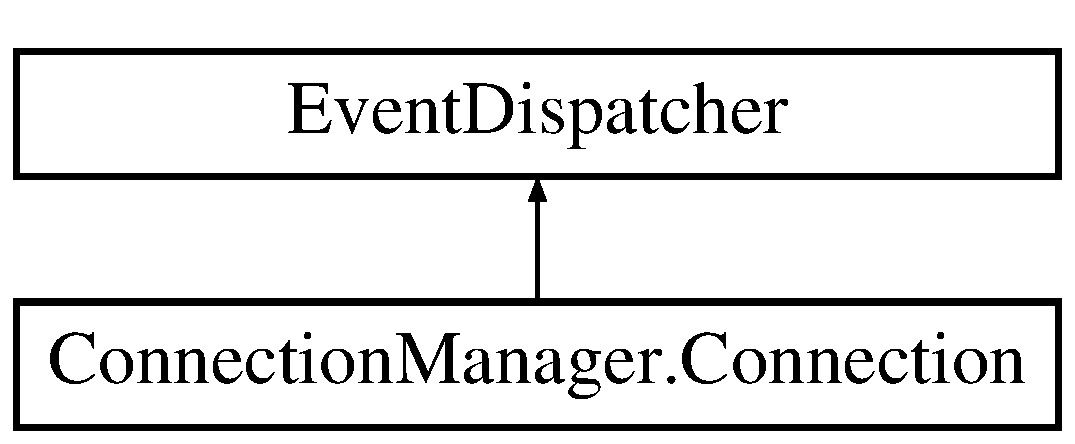
\includegraphics[height=2.000000cm]{class_connection_manager_1_1_connection}
\end{center}
\end{figure}
\subsection*{Public Member Functions}
\begin{DoxyCompactItemize}
\item 
def \hyperlink{class_connection_manager_1_1_connection_aed48556114c40be29ee0368b0aae32ac}{\-\_\-\-\_\-init\-\_\-\-\_\-}
\begin{DoxyCompactList}\small\item\em Default constructor. \end{DoxyCompactList}\item 
def \hyperlink{class_connection_manager_1_1_connection_a9b2e60752c684646830f8ce9923ee66e}{close\-\_\-connection}
\begin{DoxyCompactList}\small\item\em Close this connection. \end{DoxyCompactList}\end{DoxyCompactItemize}
\subsection*{Public Attributes}
\begin{DoxyCompactItemize}
\item 
\hyperlink{class_connection_manager_1_1_connection_acf891c29169c0404caf1941086ed8ea5}{socket}
\begin{DoxyCompactList}\small\item\em The socket associated with this connection. \end{DoxyCompactList}\item 
\hyperlink{class_connection_manager_1_1_connection_a6363bfbd5eb310be1d9d8f8f3c316a64}{input\-\_\-buffer}
\begin{DoxyCompactList}\small\item\em The input buffer where received data is stored. \end{DoxyCompactList}\item 
\hyperlink{class_connection_manager_1_1_connection_a3dcce4ca0299bef196ffb49ab2795330}{output\-\_\-buffer}
\begin{DoxyCompactList}\small\item\em The output buffer where data, which needs to be sent over the socket is stored. \end{DoxyCompactList}\item 
\hyperlink{class_connection_manager_1_1_connection_a36948dfdd00bb9b1f3d8246c874238a9}{handler}
\begin{DoxyCompactList}\small\item\em This is an instance of the Http\-Request\-Handler. \end{DoxyCompactList}\end{DoxyCompactItemize}


\subsection{Detailed Description}
Class representing a physical connection to the server. 

\subsection{Constructor \& Destructor Documentation}
\hypertarget{class_connection_manager_1_1_connection_aed48556114c40be29ee0368b0aae32ac}{\index{Connection\-Manager\-::\-Connection@{Connection\-Manager\-::\-Connection}!\-\_\-\-\_\-init\-\_\-\-\_\-@{\-\_\-\-\_\-init\-\_\-\-\_\-}}
\index{\-\_\-\-\_\-init\-\_\-\-\_\-@{\-\_\-\-\_\-init\-\_\-\-\_\-}!ConnectionManager::Connection@{Connection\-Manager\-::\-Connection}}
\subsubsection[{\-\_\-\-\_\-init\-\_\-\-\_\-}]{\setlength{\rightskip}{0pt plus 5cm}def Connection\-Manager.\-Connection.\-\_\-\-\_\-init\-\_\-\-\_\- (
\begin{DoxyParamCaption}
\item[{}]{self, }
\item[{}]{socket}
\end{DoxyParamCaption}
)}}\label{class_connection_manager_1_1_connection_aed48556114c40be29ee0368b0aae32ac}


Default constructor. 

Sets the socket associated with this connection. 
\begin{DoxyParams}{Parameters}
{\em socket} & The connection socket \\
\hline
\end{DoxyParams}


\subsection{Member Function Documentation}
\hypertarget{class_connection_manager_1_1_connection_a9b2e60752c684646830f8ce9923ee66e}{\index{Connection\-Manager\-::\-Connection@{Connection\-Manager\-::\-Connection}!close\-\_\-connection@{close\-\_\-connection}}
\index{close\-\_\-connection@{close\-\_\-connection}!ConnectionManager::Connection@{Connection\-Manager\-::\-Connection}}
\subsubsection[{close\-\_\-connection}]{\setlength{\rightskip}{0pt plus 5cm}def Connection\-Manager.\-Connection.\-close\-\_\-connection (
\begin{DoxyParamCaption}
\item[{}]{self}
\end{DoxyParamCaption}
)}}\label{class_connection_manager_1_1_connection_a9b2e60752c684646830f8ce9923ee66e}


Close this connection. 

Closes the connection by calling the close() method on the socket. 

\subsection{Member Data Documentation}
\hypertarget{class_connection_manager_1_1_connection_a36948dfdd00bb9b1f3d8246c874238a9}{\index{Connection\-Manager\-::\-Connection@{Connection\-Manager\-::\-Connection}!handler@{handler}}
\index{handler@{handler}!ConnectionManager::Connection@{Connection\-Manager\-::\-Connection}}
\subsubsection[{handler}]{\setlength{\rightskip}{0pt plus 5cm}Connection\-Manager.\-Connection.\-handler}}\label{class_connection_manager_1_1_connection_a36948dfdd00bb9b1f3d8246c874238a9}


This is an instance of the Http\-Request\-Handler. 

It is responsible for processing request and generating responses. \hypertarget{class_connection_manager_1_1_connection_a6363bfbd5eb310be1d9d8f8f3c316a64}{\index{Connection\-Manager\-::\-Connection@{Connection\-Manager\-::\-Connection}!input\-\_\-buffer@{input\-\_\-buffer}}
\index{input\-\_\-buffer@{input\-\_\-buffer}!ConnectionManager::Connection@{Connection\-Manager\-::\-Connection}}
\subsubsection[{input\-\_\-buffer}]{\setlength{\rightskip}{0pt plus 5cm}Connection\-Manager.\-Connection.\-input\-\_\-buffer}}\label{class_connection_manager_1_1_connection_a6363bfbd5eb310be1d9d8f8f3c316a64}


The input buffer where received data is stored. 

\hypertarget{class_connection_manager_1_1_connection_a3dcce4ca0299bef196ffb49ab2795330}{\index{Connection\-Manager\-::\-Connection@{Connection\-Manager\-::\-Connection}!output\-\_\-buffer@{output\-\_\-buffer}}
\index{output\-\_\-buffer@{output\-\_\-buffer}!ConnectionManager::Connection@{Connection\-Manager\-::\-Connection}}
\subsubsection[{output\-\_\-buffer}]{\setlength{\rightskip}{0pt plus 5cm}Connection\-Manager.\-Connection.\-output\-\_\-buffer}}\label{class_connection_manager_1_1_connection_a3dcce4ca0299bef196ffb49ab2795330}


The output buffer where data, which needs to be sent over the socket is stored. 

\hypertarget{class_connection_manager_1_1_connection_acf891c29169c0404caf1941086ed8ea5}{\index{Connection\-Manager\-::\-Connection@{Connection\-Manager\-::\-Connection}!socket@{socket}}
\index{socket@{socket}!ConnectionManager::Connection@{Connection\-Manager\-::\-Connection}}
\subsubsection[{socket}]{\setlength{\rightskip}{0pt plus 5cm}Connection\-Manager.\-Connection.\-socket}}\label{class_connection_manager_1_1_connection_acf891c29169c0404caf1941086ed8ea5}


The socket associated with this connection. 



The documentation for this class was generated from the following file\-:\begin{DoxyCompactItemize}
\item 
/home/ivan/\-Code\-Snippets-\/\-Projects/\-Telebid-\/\-Tasks/\-Web\-Server/\-Async\-Server/Connection\-Manager.\-py\end{DoxyCompactItemize}

\hypertarget{class_connection_manager_1_1_connection_manager}{\section{Connection\-Manager.\-Connection\-Manager Class Reference}
\label{class_connection_manager_1_1_connection_manager}\index{Connection\-Manager.\-Connection\-Manager@{Connection\-Manager.\-Connection\-Manager}}
}


Class used for managing active connections.  


Inheritance diagram for Connection\-Manager.\-Connection\-Manager\-:\begin{figure}[H]
\begin{center}
\leavevmode
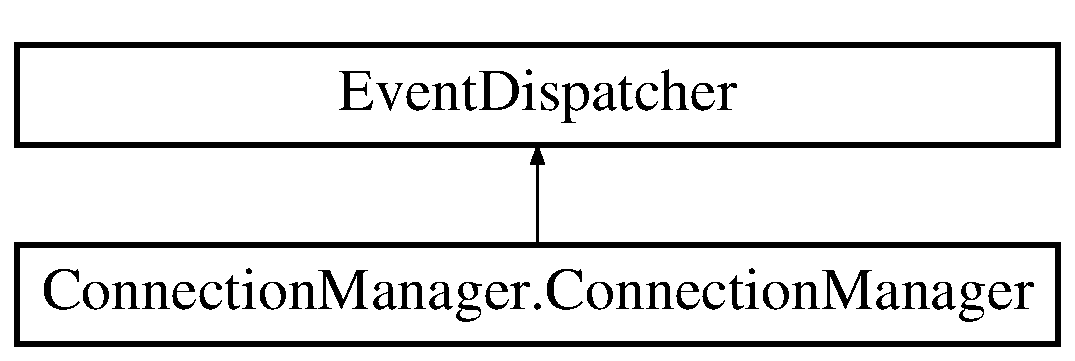
\includegraphics[height=2.000000cm]{class_connection_manager_1_1_connection_manager}
\end{center}
\end{figure}
\subsection*{Public Member Functions}
\begin{DoxyCompactItemize}
\item 
\hypertarget{class_connection_manager_1_1_connection_manager_af1b9f53192d93384ed9cb52b265ff0fd}{def \hyperlink{class_connection_manager_1_1_connection_manager_af1b9f53192d93384ed9cb52b265ff0fd}{\-\_\-\-\_\-init\-\_\-\-\_\-}}\label{class_connection_manager_1_1_connection_manager_af1b9f53192d93384ed9cb52b265ff0fd}

\begin{DoxyCompactList}\small\item\em Default constructor. \end{DoxyCompactList}\item 
def \hyperlink{class_connection_manager_1_1_connection_manager_a4a36c1328d67eacf11ea3ad11a892751}{handle\-\_\-event}
\begin{DoxyCompactList}\small\item\em Method inherited from Event\-Handler class. \end{DoxyCompactList}\item 
def \hyperlink{class_connection_manager_1_1_connection_manager_a36acc18652824eb9d1c23818ed55effb}{find\-\_\-connection}
\begin{DoxyCompactList}\small\item\em Iterate through the list of connections and search for a connection associated with socket. \end{DoxyCompactList}\end{DoxyCompactItemize}
\subsection*{Public Attributes}
\begin{DoxyCompactItemize}
\item 
\hyperlink{class_connection_manager_1_1_connection_manager_a0c355961ff6a71c3e50b3ed112b8c536}{connections}
\begin{DoxyCompactList}\small\item\em List of active connections. \end{DoxyCompactList}\end{DoxyCompactItemize}


\subsection{Detailed Description}
Class used for managing active connections. 

This class is responsible for creating, destroying and updating physical connections. 

\subsection{Member Function Documentation}
\hypertarget{class_connection_manager_1_1_connection_manager_a36acc18652824eb9d1c23818ed55effb}{\index{Connection\-Manager\-::\-Connection\-Manager@{Connection\-Manager\-::\-Connection\-Manager}!find\-\_\-connection@{find\-\_\-connection}}
\index{find\-\_\-connection@{find\-\_\-connection}!ConnectionManager::ConnectionManager@{Connection\-Manager\-::\-Connection\-Manager}}
\subsubsection[{find\-\_\-connection}]{\setlength{\rightskip}{0pt plus 5cm}def Connection\-Manager.\-Connection\-Manager.\-find\-\_\-connection (
\begin{DoxyParamCaption}
\item[{}]{self, }
\item[{}]{socket}
\end{DoxyParamCaption}
)}}\label{class_connection_manager_1_1_connection_manager_a36acc18652824eb9d1c23818ed55effb}


Iterate through the list of connections and search for a connection associated with socket. 

If the function succeeds it returns the connection object associated with the socket. If no such connection is found, the function returns None.


\begin{DoxyParams}{Parameters}
{\em socket} & The socket to search for. \\
\hline
\end{DoxyParams}
\begin{DoxyReturn}{Returns}
\hyperlink{class_connection_manager_1_1_connection}{Connection} object associated with socket or {\bfseries None} if no such connection was found. 
\end{DoxyReturn}
\hypertarget{class_connection_manager_1_1_connection_manager_a4a36c1328d67eacf11ea3ad11a892751}{\index{Connection\-Manager\-::\-Connection\-Manager@{Connection\-Manager\-::\-Connection\-Manager}!handle\-\_\-event@{handle\-\_\-event}}
\index{handle\-\_\-event@{handle\-\_\-event}!ConnectionManager::ConnectionManager@{Connection\-Manager\-::\-Connection\-Manager}}
\subsubsection[{handle\-\_\-event}]{\setlength{\rightskip}{0pt plus 5cm}def Connection\-Manager.\-Connection\-Manager.\-handle\-\_\-event (
\begin{DoxyParamCaption}
\item[{}]{self, }
\item[{}]{event}
\end{DoxyParamCaption}
)}}\label{class_connection_manager_1_1_connection_manager_a4a36c1328d67eacf11ea3ad11a892751}


Method inherited from Event\-Handler class. 

This is where the main logic of the class is realised. This method is called by the Web\-Server class each time it submits an event. Here we create new Connections objects when a connection is established, we close connections which are no longer active and process received data.


\begin{DoxyParams}{Parameters}
{\em event} & The event that triggered this function. \\
\hline
\end{DoxyParams}


\subsection{Member Data Documentation}
\hypertarget{class_connection_manager_1_1_connection_manager_a0c355961ff6a71c3e50b3ed112b8c536}{\index{Connection\-Manager\-::\-Connection\-Manager@{Connection\-Manager\-::\-Connection\-Manager}!connections@{connections}}
\index{connections@{connections}!ConnectionManager::ConnectionManager@{Connection\-Manager\-::\-Connection\-Manager}}
\subsubsection[{connections}]{\setlength{\rightskip}{0pt plus 5cm}Connection\-Manager.\-Connection\-Manager.\-connections}}\label{class_connection_manager_1_1_connection_manager_a0c355961ff6a71c3e50b3ed112b8c536}


List of active connections. 



The documentation for this class was generated from the following file\-:\begin{DoxyCompactItemize}
\item 
/home/ivan/\-Code\-Snippets-\/\-Projects/\-Telebid-\/\-Tasks/\-Web\-Server/\-Async\-Server/Connection\-Manager.\-py\end{DoxyCompactItemize}

\hypertarget{class_event_dispatcher_1_1_entry}{\section{Event\-Dispatcher.\-Entry Class Reference}
\label{class_event_dispatcher_1_1_entry}\index{Event\-Dispatcher.\-Entry@{Event\-Dispatcher.\-Entry}}
}


Class representing a (handler, event code) pair.  


Inheritance diagram for Event\-Dispatcher.\-Entry\-:\begin{figure}[H]
\begin{center}
\leavevmode
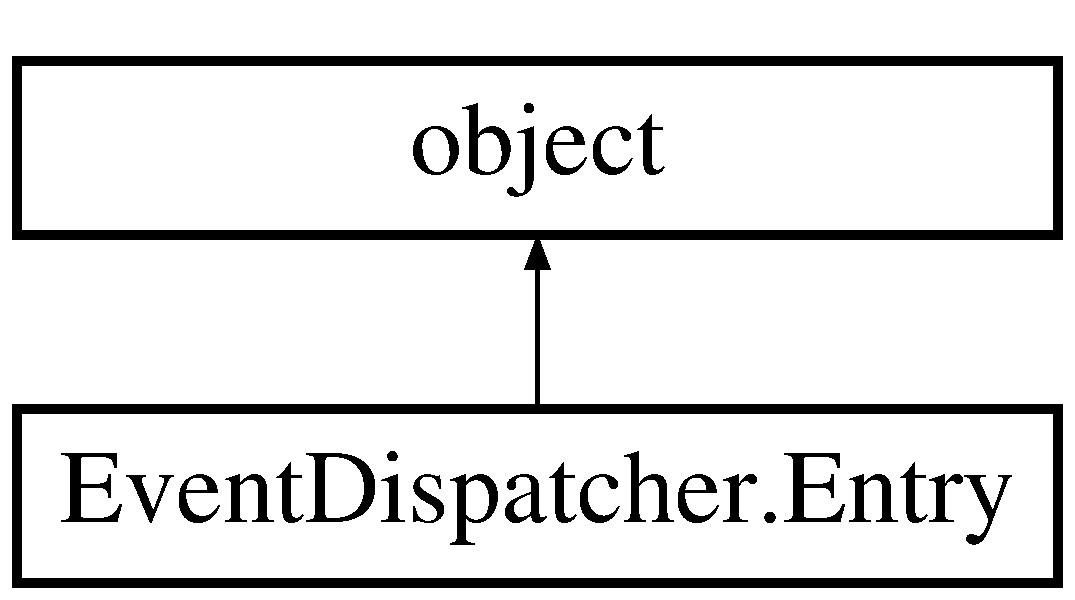
\includegraphics[height=2.000000cm]{class_event_dispatcher_1_1_entry}
\end{center}
\end{figure}
\subsection*{Public Member Functions}
\begin{DoxyCompactItemize}
\item 
\hypertarget{class_event_dispatcher_1_1_entry_ac1a11d896e644420b9fb175c6ff284bc}{def \hyperlink{class_event_dispatcher_1_1_entry_ac1a11d896e644420b9fb175c6ff284bc}{\-\_\-\-\_\-init\-\_\-\-\_\-}}\label{class_event_dispatcher_1_1_entry_ac1a11d896e644420b9fb175c6ff284bc}

\begin{DoxyCompactList}\small\item\em Default constructor. \end{DoxyCompactList}\end{DoxyCompactItemize}
\subsection*{Public Attributes}
\begin{DoxyCompactItemize}
\item 
\hypertarget{class_event_dispatcher_1_1_entry_ae7db320cec210a771ec6b058e12b336b}{{\bfseries handler}}\label{class_event_dispatcher_1_1_entry_ae7db320cec210a771ec6b058e12b336b}

\item 
\hypertarget{class_event_dispatcher_1_1_entry_a8c2ab6901f00ec0edc1256d37be91630}{{\bfseries code}}\label{class_event_dispatcher_1_1_entry_a8c2ab6901f00ec0edc1256d37be91630}

\end{DoxyCompactItemize}


\subsection{Detailed Description}
Class representing a (handler, event code) pair. 

This class is internally used by the \hyperlink{class_event_dispatcher_1_1_event_dispatcher}{Event\-Dispatcher} class to maintain a list of event handlers. Each event handler is associated with the event code it is listening for. 

The documentation for this class was generated from the following file\-:\begin{DoxyCompactItemize}
\item 
/home/ivan/\-Code\-Snippets-\/\-Projects/\-Telebid-\/\-Tasks/\-Web\-Server/\-Async\-Server/Event\-Dispatcher.\-py\end{DoxyCompactItemize}

\hypertarget{class_event_dispatcher_1_1_event}{\section{Event\-Dispatcher.\-Event Class Reference}
\label{class_event_dispatcher_1_1_event}\index{Event\-Dispatcher.\-Event@{Event\-Dispatcher.\-Event}}
}


Class representing an event.  


Inheritance diagram for Event\-Dispatcher.\-Event\-:\begin{figure}[H]
\begin{center}
\leavevmode
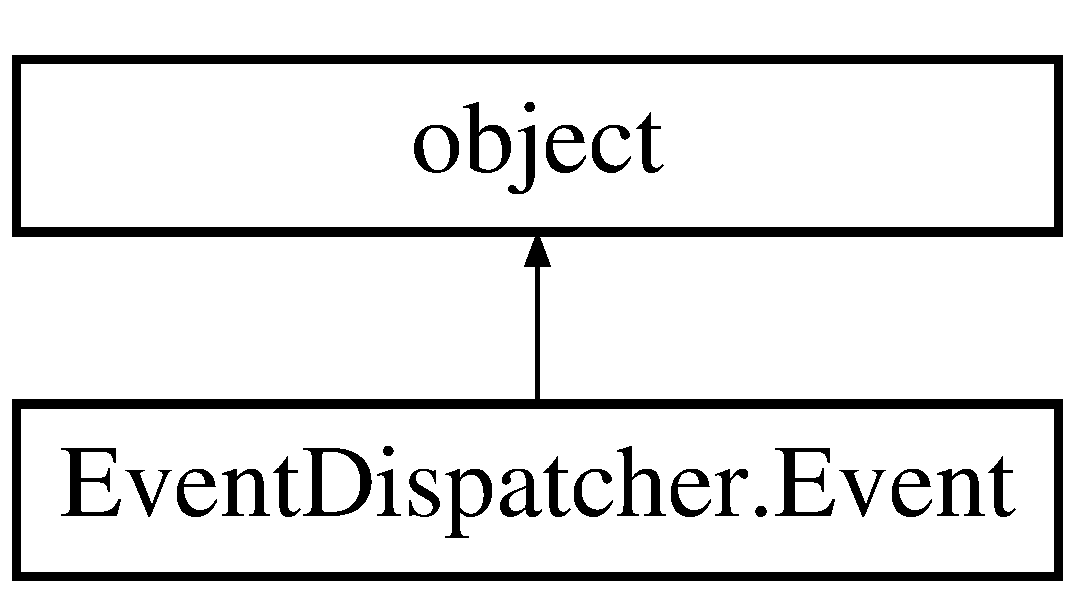
\includegraphics[height=2.000000cm]{class_event_dispatcher_1_1_event}
\end{center}
\end{figure}
\subsection*{Public Member Functions}
\begin{DoxyCompactItemize}
\item 
\hypertarget{class_event_dispatcher_1_1_event_a7b12495347b4eb0c5b44f8b6749de7a0}{def \hyperlink{class_event_dispatcher_1_1_event_a7b12495347b4eb0c5b44f8b6749de7a0}{\-\_\-\-\_\-init\-\_\-\-\_\-}}\label{class_event_dispatcher_1_1_event_a7b12495347b4eb0c5b44f8b6749de7a0}

\begin{DoxyCompactList}\small\item\em Default constructor. \end{DoxyCompactList}\end{DoxyCompactItemize}
\subsection*{Public Attributes}
\begin{DoxyCompactItemize}
\item 
\hypertarget{class_event_dispatcher_1_1_event_aa87c86a13babd2b77d234f5d6d91feaa}{{\bfseries code}}\label{class_event_dispatcher_1_1_event_aa87c86a13babd2b77d234f5d6d91feaa}

\item 
\hypertarget{class_event_dispatcher_1_1_event_a254ec16bd2f1e54bd2767d35d2cbb976}{{\bfseries data}}\label{class_event_dispatcher_1_1_event_a254ec16bd2f1e54bd2767d35d2cbb976}

\end{DoxyCompactItemize}
\subsection*{Static Public Attributes}
\begin{DoxyCompactItemize}
\item 
\hypertarget{class_event_dispatcher_1_1_event_a5ca59aecfeb4d82115c7aac7fa8d2593}{int {\bfseries N\-U\-L\-L} = 0}\label{class_event_dispatcher_1_1_event_a5ca59aecfeb4d82115c7aac7fa8d2593}

\item 
\hypertarget{class_event_dispatcher_1_1_event_ab9e67d0ed999cbe39bbe3192646ba53f}{int {\bfseries N\-E\-T\-W\-O\-R\-K\-\_\-\-C\-O\-N\-N\-E\-C\-T} = 2}\label{class_event_dispatcher_1_1_event_ab9e67d0ed999cbe39bbe3192646ba53f}

\item 
\hypertarget{class_event_dispatcher_1_1_event_ad19d0d6232f81c72950eb2323e103042}{int {\bfseries N\-E\-T\-W\-O\-R\-K\-\_\-\-D\-I\-S\-C\-O\-N\-N\-E\-C\-T} = 3}\label{class_event_dispatcher_1_1_event_ad19d0d6232f81c72950eb2323e103042}

\item 
\hypertarget{class_event_dispatcher_1_1_event_a2a7032f1a9f61847dbe4d1b8809e9771}{int {\bfseries N\-E\-T\-W\-O\-R\-K\-\_\-\-D\-A\-T\-A} = 4}\label{class_event_dispatcher_1_1_event_a2a7032f1a9f61847dbe4d1b8809e9771}

\item 
\hypertarget{class_event_dispatcher_1_1_event_a01ca1da93062191cc6df96602c5036ae}{int {\bfseries R\-E\-C\-E\-I\-V\-E\-D\-\_\-\-R\-E\-Q\-U\-E\-S\-T} = 6}\label{class_event_dispatcher_1_1_event_a01ca1da93062191cc6df96602c5036ae}

\item 
\hypertarget{class_event_dispatcher_1_1_event_ac547b813d72336971dc9b6fb0b4b3c2f}{int {\bfseries T\-A\-S\-K\-\_\-\-S\-T\-A\-R\-T} = 7}\label{class_event_dispatcher_1_1_event_ac547b813d72336971dc9b6fb0b4b3c2f}

\item 
\hypertarget{class_event_dispatcher_1_1_event_ae53f46e531b4c0dfa05396cb7d457bfb}{int {\bfseries T\-A\-S\-K\-\_\-\-U\-P\-D\-A\-T\-E} = 8}\label{class_event_dispatcher_1_1_event_ae53f46e531b4c0dfa05396cb7d457bfb}

\item 
\hypertarget{class_event_dispatcher_1_1_event_a93ae5c1e018c498e8dc803fca32bdc03}{int {\bfseries T\-A\-S\-K\-\_\-\-D\-O\-N\-E} = 9}\label{class_event_dispatcher_1_1_event_a93ae5c1e018c498e8dc803fca32bdc03}

\item 
\hypertarget{class_event_dispatcher_1_1_event_af631bd478bb4e2992539eb3cdd3773ed}{int {\bfseries T\-A\-S\-K\-\_\-\-D\-A\-T\-A} = 10}\label{class_event_dispatcher_1_1_event_af631bd478bb4e2992539eb3cdd3773ed}

\end{DoxyCompactItemize}


\subsection{Detailed Description}
Class representing an event. 

Each event has a code, which is used by the \hyperlink{class_event_dispatcher_1_1_event_dispatcher}{Event\-Dispatcher} to determine which handler to invoke when calling the dispatch\-\_\-event() method. The \hyperlink{class_event_dispatcher_1_1_event}{Event} class has a field name data. It is used to transmit additional data along with the event. 

The documentation for this class was generated from the following file\-:\begin{DoxyCompactItemize}
\item 
/home/ivan/\-Code\-Snippets-\/\-Projects/\-Telebid-\/\-Tasks/\-Web\-Server/\-Async\-Server/Event\-Dispatcher.\-py\end{DoxyCompactItemize}

\hypertarget{class_event_dispatcher_1_1_event_dispatcher}{\section{Event\-Dispatcher.\-Event\-Dispatcher Class Reference}
\label{class_event_dispatcher_1_1_event_dispatcher}\index{Event\-Dispatcher.\-Event\-Dispatcher@{Event\-Dispatcher.\-Event\-Dispatcher}}
}


The \hyperlink{class_event_dispatcher_1_1_event_dispatcher}{Event\-Dispatcher} class is used for dispatching events.  


Inheritance diagram for Event\-Dispatcher.\-Event\-Dispatcher\-:\begin{figure}[H]
\begin{center}
\leavevmode
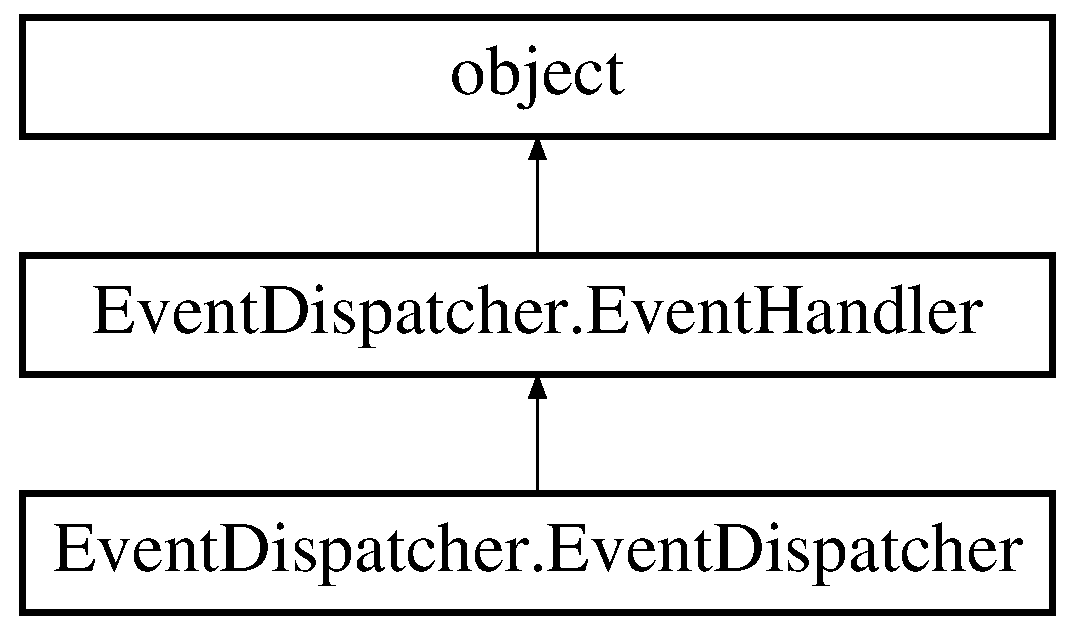
\includegraphics[height=3.000000cm]{class_event_dispatcher_1_1_event_dispatcher}
\end{center}
\end{figure}
\subsection*{Public Member Functions}
\begin{DoxyCompactItemize}
\item 
\hypertarget{class_event_dispatcher_1_1_event_dispatcher_abeca2b40e540e444eb96a233a9c697d9}{def \hyperlink{class_event_dispatcher_1_1_event_dispatcher_abeca2b40e540e444eb96a233a9c697d9}{\-\_\-\-\_\-init\-\_\-\-\_\-}}\label{class_event_dispatcher_1_1_event_dispatcher_abeca2b40e540e444eb96a233a9c697d9}

\begin{DoxyCompactList}\small\item\em Default constructor. \end{DoxyCompactList}\item 
def \hyperlink{class_event_dispatcher_1_1_event_dispatcher_accf2a074566d17035a7505fbd428dc29}{has\-\_\-event\-\_\-listener}
\begin{DoxyCompactList}\small\item\em Checks to see if a given \hyperlink{class_event_dispatcher_1_1_event_handler}{Event\-Handler} is already associated with a given event code. \end{DoxyCompactList}\item 
def \hyperlink{class_event_dispatcher_1_1_event_dispatcher_ae1fe43c67bf61743f8689fc13354fe22}{add\-\_\-event\-\_\-listener}
\begin{DoxyCompactList}\small\item\em Register an \hyperlink{class_event_dispatcher_1_1_event_handler}{Event\-Handler} to listen for an \hyperlink{class_event_dispatcher_1_1_event}{Event} with code code. \end{DoxyCompactList}\item 
def \hyperlink{class_event_dispatcher_1_1_event_dispatcher_abc78a2a5438b435e11a3f11f51aeabf5}{remove\-\_\-event\-\_\-listener}
\begin{DoxyCompactList}\small\item\em Stop an \hyperlink{class_event_dispatcher_1_1_event_handler}{Event\-Handler} from listening for a specific \hyperlink{class_event_dispatcher_1_1_event}{Event} with code code. \end{DoxyCompactList}\item 
def \hyperlink{class_event_dispatcher_1_1_event_dispatcher_a79463708a50cf97ca6ef39c8004d5550}{remove\-\_\-event\-\_\-listener\-\_\-all}
\begin{DoxyCompactList}\small\item\em Stops a given \hyperlink{class_event_dispatcher_1_1_event_handler}{Event\-Handler} from listening to all event codes. \end{DoxyCompactList}\item 
def \hyperlink{class_event_dispatcher_1_1_event_dispatcher_af7ba3f3cb530002c126735f2b76ab05f}{dispatch\-\_\-event}
\begin{DoxyCompactList}\small\item\em Dispatch an event to all Event\-Handlers listening for that \hyperlink{class_event_dispatcher_1_1_event}{Event}. \end{DoxyCompactList}\end{DoxyCompactItemize}
\subsection*{Public Attributes}
\begin{DoxyCompactItemize}
\item 
\hypertarget{class_event_dispatcher_1_1_event_dispatcher_a81d42028fa864b144c92df04268ca4e7}{\hyperlink{class_event_dispatcher_1_1_event_dispatcher_a81d42028fa864b144c92df04268ca4e7}{handlers}}\label{class_event_dispatcher_1_1_event_dispatcher_a81d42028fa864b144c92df04268ca4e7}

\begin{DoxyCompactList}\small\item\em List of registered Event\-Handlers. \end{DoxyCompactList}\end{DoxyCompactItemize}


\subsection{Detailed Description}
The \hyperlink{class_event_dispatcher_1_1_event_dispatcher}{Event\-Dispatcher} class is used for dispatching events. 

To give a class the ability to send and receive events all you need to do is inherit this class. 

\subsection{Member Function Documentation}
\hypertarget{class_event_dispatcher_1_1_event_dispatcher_ae1fe43c67bf61743f8689fc13354fe22}{\index{Event\-Dispatcher\-::\-Event\-Dispatcher@{Event\-Dispatcher\-::\-Event\-Dispatcher}!add\-\_\-event\-\_\-listener@{add\-\_\-event\-\_\-listener}}
\index{add\-\_\-event\-\_\-listener@{add\-\_\-event\-\_\-listener}!EventDispatcher::EventDispatcher@{Event\-Dispatcher\-::\-Event\-Dispatcher}}
\subsubsection[{add\-\_\-event\-\_\-listener}]{\setlength{\rightskip}{0pt plus 5cm}def Event\-Dispatcher.\-Event\-Dispatcher.\-add\-\_\-event\-\_\-listener (
\begin{DoxyParamCaption}
\item[{}]{self, }
\item[{}]{handler, }
\item[{}]{code}
\end{DoxyParamCaption}
)}}\label{class_event_dispatcher_1_1_event_dispatcher_ae1fe43c67bf61743f8689fc13354fe22}


Register an \hyperlink{class_event_dispatcher_1_1_event_handler}{Event\-Handler} to listen for an \hyperlink{class_event_dispatcher_1_1_event}{Event} with code code. 


\begin{DoxyParams}{Parameters}
{\em handler} & Handler to register, \\
\hline
{\em code} & \hyperlink{class_event_dispatcher_1_1_event}{Event} code that this handler is listening for. \\
\hline
\end{DoxyParams}
\hypertarget{class_event_dispatcher_1_1_event_dispatcher_af7ba3f3cb530002c126735f2b76ab05f}{\index{Event\-Dispatcher\-::\-Event\-Dispatcher@{Event\-Dispatcher\-::\-Event\-Dispatcher}!dispatch\-\_\-event@{dispatch\-\_\-event}}
\index{dispatch\-\_\-event@{dispatch\-\_\-event}!EventDispatcher::EventDispatcher@{Event\-Dispatcher\-::\-Event\-Dispatcher}}
\subsubsection[{dispatch\-\_\-event}]{\setlength{\rightskip}{0pt plus 5cm}def Event\-Dispatcher.\-Event\-Dispatcher.\-dispatch\-\_\-event (
\begin{DoxyParamCaption}
\item[{}]{self, }
\item[{}]{event}
\end{DoxyParamCaption}
)}}\label{class_event_dispatcher_1_1_event_dispatcher_af7ba3f3cb530002c126735f2b76ab05f}


Dispatch an event to all Event\-Handlers listening for that \hyperlink{class_event_dispatcher_1_1_event}{Event}. 


\begin{DoxyParams}{Parameters}
{\em event} & \hyperlink{class_event_dispatcher_1_1_event}{Event} which to dispatch. \\
\hline
\end{DoxyParams}
\hypertarget{class_event_dispatcher_1_1_event_dispatcher_accf2a074566d17035a7505fbd428dc29}{\index{Event\-Dispatcher\-::\-Event\-Dispatcher@{Event\-Dispatcher\-::\-Event\-Dispatcher}!has\-\_\-event\-\_\-listener@{has\-\_\-event\-\_\-listener}}
\index{has\-\_\-event\-\_\-listener@{has\-\_\-event\-\_\-listener}!EventDispatcher::EventDispatcher@{Event\-Dispatcher\-::\-Event\-Dispatcher}}
\subsubsection[{has\-\_\-event\-\_\-listener}]{\setlength{\rightskip}{0pt plus 5cm}def Event\-Dispatcher.\-Event\-Dispatcher.\-has\-\_\-event\-\_\-listener (
\begin{DoxyParamCaption}
\item[{}]{self, }
\item[{}]{handler, }
\item[{}]{code}
\end{DoxyParamCaption}
)}}\label{class_event_dispatcher_1_1_event_dispatcher_accf2a074566d17035a7505fbd428dc29}


Checks to see if a given \hyperlink{class_event_dispatcher_1_1_event_handler}{Event\-Handler} is already associated with a given event code. 


\begin{DoxyParams}{Parameters}
{\em handler} & The \hyperlink{class_event_dispatcher_1_1_event_handler}{Event\-Handler} to check for. \\
\hline
{\em code} & The event code to check for. \\
\hline
\end{DoxyParams}
\begin{DoxyReturn}{Returns}
True is the \hyperlink{class_event_dispatcher_1_1_event_handler}{Event\-Handler} is already associated to the event code and False otherwis 
\end{DoxyReturn}
\hypertarget{class_event_dispatcher_1_1_event_dispatcher_abc78a2a5438b435e11a3f11f51aeabf5}{\index{Event\-Dispatcher\-::\-Event\-Dispatcher@{Event\-Dispatcher\-::\-Event\-Dispatcher}!remove\-\_\-event\-\_\-listener@{remove\-\_\-event\-\_\-listener}}
\index{remove\-\_\-event\-\_\-listener@{remove\-\_\-event\-\_\-listener}!EventDispatcher::EventDispatcher@{Event\-Dispatcher\-::\-Event\-Dispatcher}}
\subsubsection[{remove\-\_\-event\-\_\-listener}]{\setlength{\rightskip}{0pt plus 5cm}def Event\-Dispatcher.\-Event\-Dispatcher.\-remove\-\_\-event\-\_\-listener (
\begin{DoxyParamCaption}
\item[{}]{self, }
\item[{}]{handler, }
\item[{}]{code}
\end{DoxyParamCaption}
)}}\label{class_event_dispatcher_1_1_event_dispatcher_abc78a2a5438b435e11a3f11f51aeabf5}


Stop an \hyperlink{class_event_dispatcher_1_1_event_handler}{Event\-Handler} from listening for a specific \hyperlink{class_event_dispatcher_1_1_event}{Event} with code code. 


\begin{DoxyParams}{Parameters}
{\em handler} & \hyperlink{class_event_dispatcher_1_1_event_handler}{Event\-Handler} to remove. \\
\hline
{\em code} & \hyperlink{class_event_dispatcher_1_1_event}{Event} code to remove. \\
\hline
\end{DoxyParams}
\hypertarget{class_event_dispatcher_1_1_event_dispatcher_a79463708a50cf97ca6ef39c8004d5550}{\index{Event\-Dispatcher\-::\-Event\-Dispatcher@{Event\-Dispatcher\-::\-Event\-Dispatcher}!remove\-\_\-event\-\_\-listener\-\_\-all@{remove\-\_\-event\-\_\-listener\-\_\-all}}
\index{remove\-\_\-event\-\_\-listener\-\_\-all@{remove\-\_\-event\-\_\-listener\-\_\-all}!EventDispatcher::EventDispatcher@{Event\-Dispatcher\-::\-Event\-Dispatcher}}
\subsubsection[{remove\-\_\-event\-\_\-listener\-\_\-all}]{\setlength{\rightskip}{0pt plus 5cm}def Event\-Dispatcher.\-Event\-Dispatcher.\-remove\-\_\-event\-\_\-listener\-\_\-all (
\begin{DoxyParamCaption}
\item[{}]{self, }
\item[{}]{handler}
\end{DoxyParamCaption}
)}}\label{class_event_dispatcher_1_1_event_dispatcher_a79463708a50cf97ca6ef39c8004d5550}


Stops a given \hyperlink{class_event_dispatcher_1_1_event_handler}{Event\-Handler} from listening to all event codes. 


\begin{DoxyParams}{Parameters}
{\em handler} & The \hyperlink{class_event_dispatcher_1_1_event_handler}{Event\-Handler} to remove. \\
\hline
\end{DoxyParams}


The documentation for this class was generated from the following file\-:\begin{DoxyCompactItemize}
\item 
/home/ivan/\-Code\-Snippets-\/\-Projects/\-Telebid-\/\-Tasks/\-Web\-Server/\-Async\-Server/Event\-Dispatcher.\-py\end{DoxyCompactItemize}

\hypertarget{class_event_dispatcher_1_1_event_handler}{\section{Event\-Dispatcher.\-Event\-Handler Class Reference}
\label{class_event_dispatcher_1_1_event_handler}\index{Event\-Dispatcher.\-Event\-Handler@{Event\-Dispatcher.\-Event\-Handler}}
}


Abstract class for event handlers.  


Inheritance diagram for Event\-Dispatcher.\-Event\-Handler\-:\begin{figure}[H]
\begin{center}
\leavevmode
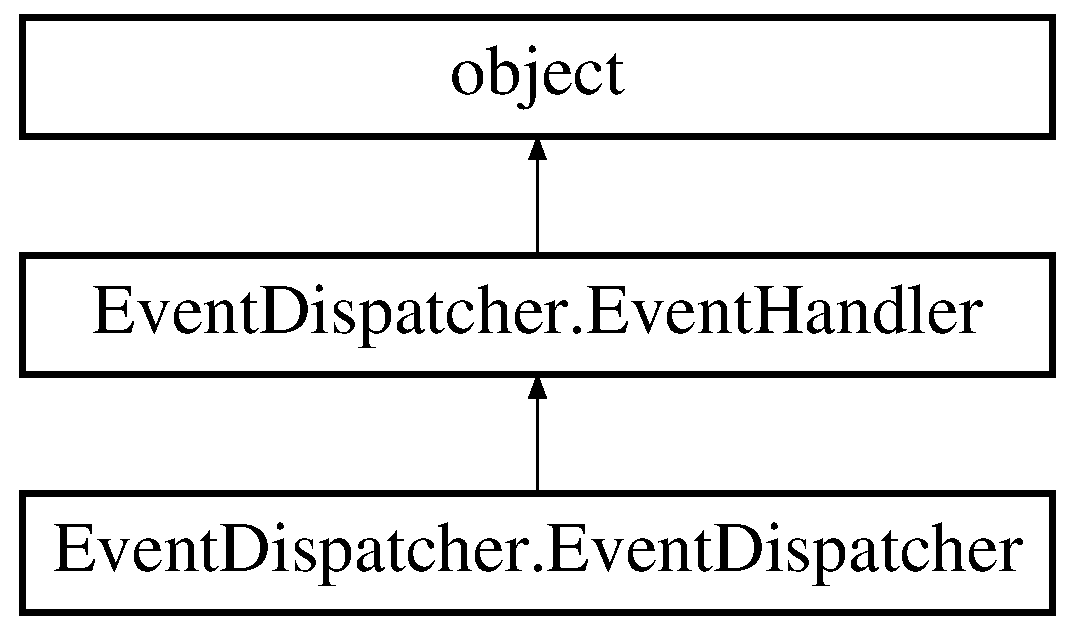
\includegraphics[height=3.000000cm]{class_event_dispatcher_1_1_event_handler}
\end{center}
\end{figure}
\subsection*{Public Member Functions}
\begin{DoxyCompactItemize}
\item 
def \hyperlink{class_event_dispatcher_1_1_event_handler_a3bb939e88fbffb1671c192e77430fa7b}{handle\-\_\-event}
\begin{DoxyCompactList}\small\item\em Method called when a certain event occurs. \end{DoxyCompactList}\end{DoxyCompactItemize}


\subsection{Detailed Description}
Abstract class for event handlers. 

You do not need to inherit this class to be able to receive messages. All you need to do is inherit \hyperlink{class_event_dispatcher_1_1_event_dispatcher}{Event\-Dispatcher} and after that you will be able to send and receive messages. 

\subsection{Member Function Documentation}
\hypertarget{class_event_dispatcher_1_1_event_handler_a3bb939e88fbffb1671c192e77430fa7b}{\index{Event\-Dispatcher\-::\-Event\-Handler@{Event\-Dispatcher\-::\-Event\-Handler}!handle\-\_\-event@{handle\-\_\-event}}
\index{handle\-\_\-event@{handle\-\_\-event}!EventDispatcher::EventHandler@{Event\-Dispatcher\-::\-Event\-Handler}}
\subsubsection[{handle\-\_\-event}]{\setlength{\rightskip}{0pt plus 5cm}def Event\-Dispatcher.\-Event\-Handler.\-handle\-\_\-event (
\begin{DoxyParamCaption}
\item[{}]{self, }
\item[{}]{event}
\end{DoxyParamCaption}
)}}\label{class_event_dispatcher_1_1_event_handler_a3bb939e88fbffb1671c192e77430fa7b}


Method called when a certain event occurs. 


\begin{DoxyParams}{Parameters}
{\em event} & The event that occurred. \\
\hline
\end{DoxyParams}


The documentation for this class was generated from the following file\-:\begin{DoxyCompactItemize}
\item 
/home/ivan/\-Code\-Snippets-\/\-Projects/\-Telebid-\/\-Tasks/\-Web\-Server/\-Async\-Server/Event\-Dispatcher.\-py\end{DoxyCompactItemize}

\hypertarget{class_http_request_1_1_http_request}{\section{Http\-Request.\-Http\-Request Class Reference}
\label{class_http_request_1_1_http_request}\index{Http\-Request.\-Http\-Request@{Http\-Request.\-Http\-Request}}
}


This class represents an Http-\/\-Request to a server.  


Inheritance diagram for Http\-Request.\-Http\-Request\-:\begin{figure}[H]
\begin{center}
\leavevmode
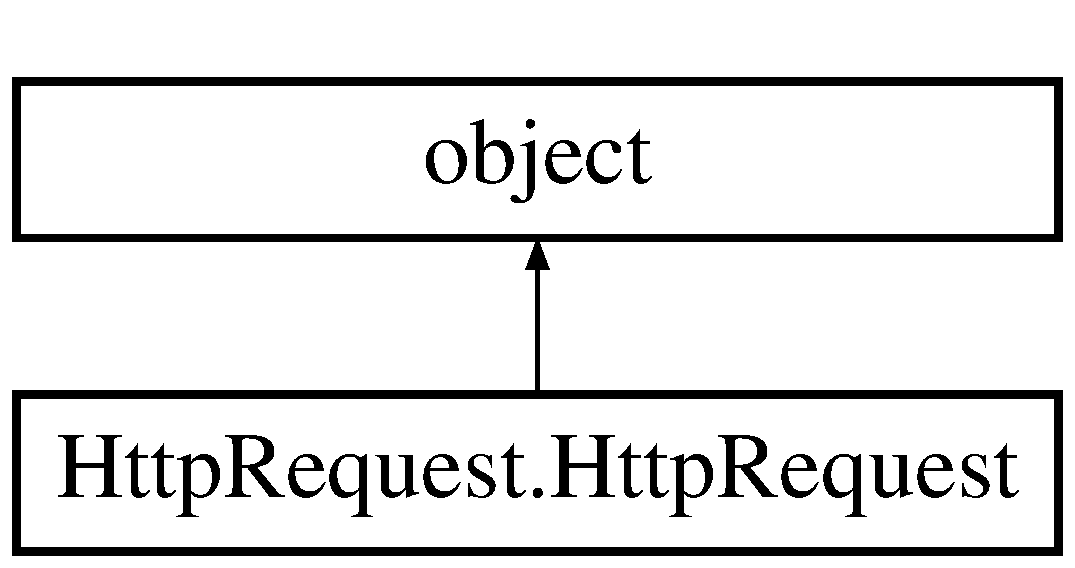
\includegraphics[height=2.000000cm]{class_http_request_1_1_http_request}
\end{center}
\end{figure}
\subsection*{Public Member Functions}
\begin{DoxyCompactItemize}
\item 
def \hyperlink{class_http_request_1_1_http_request_afdee625d1e83a73a7b2a4bb74f3b2c21}{\-\_\-\-\_\-init\-\_\-\-\_\-}
\begin{DoxyCompactList}\small\item\em Default constructor. \end{DoxyCompactList}\item 
\hypertarget{class_http_request_1_1_http_request_ad70cacde587c703f570e124aca5cca26}{def \hyperlink{class_http_request_1_1_http_request_ad70cacde587c703f570e124aca5cca26}{dump}}\label{class_http_request_1_1_http_request_ad70cacde587c703f570e124aca5cca26}

\begin{DoxyCompactList}\small\item\em Print the response to the console. \end{DoxyCompactList}\end{DoxyCompactItemize}
\subsection*{Public Attributes}
\begin{DoxyCompactItemize}
\item 
\hyperlink{class_http_request_1_1_http_request_a37deed6d8791b240c1db458c0f3eb95d}{content\-Encoding}
\begin{DoxyCompactList}\small\item\em The character set of the entity-\/body. \end{DoxyCompactList}\item 
\hyperlink{class_http_request_1_1_http_request_aa37faef2bdb70d29c6ce741d7362dad4}{content\-Length}
\begin{DoxyCompactList}\small\item\em The length, in bytes, of content sent by the client. \end{DoxyCompactList}\item 
\hyperlink{class_http_request_1_1_http_request_a588d3bb83d3d30c0de69c7175d9500ba}{content\-\_\-type}
\begin{DoxyCompactList}\small\item\em M\-I\-M\-E content type of the request. \end{DoxyCompactList}\item 
\hyperlink{class_http_request_1_1_http_request_a64b3bf1ae5347ad8570527ec6c390897}{cookies}
\begin{DoxyCompactList}\small\item\em A collection of cookies sent by the client. \end{DoxyCompactList}\item 
\hyperlink{class_http_request_1_1_http_request_a7e77838e0ad5a1dbc61cc2a5eba94fad}{form}
\begin{DoxyCompactList}\small\item\em Collection of form variables. \end{DoxyCompactList}\item 
\hyperlink{class_http_request_1_1_http_request_ab06f3b22757af971c0958d6d73028c11}{headers}
\begin{DoxyCompactList}\small\item\em Collection of H\-T\-T\-P headers. \end{DoxyCompactList}\item 
\hyperlink{class_http_request_1_1_http_request_a2ef110e9c384476bc8b20d52b075911a}{method}
\begin{DoxyCompactList}\small\item\em The H\-T\-T\-P data transfer method (such as G\-E\-T, P\-O\-S\-T, or H\-E\-A\-D) used by the client. \end{DoxyCompactList}\item 
\hyperlink{class_http_request_1_1_http_request_a1036f16b31416b249633c275ea53bfbf}{query\-\_\-strings}
\begin{DoxyCompactList}\small\item\em A collection of H\-T\-T\-P query string variables. \end{DoxyCompactList}\item 
\hyperlink{class_http_request_1_1_http_request_a4b7fa1c7de17ba07e72d76318a91d620}{referrer}
\begin{DoxyCompactList}\small\item\em Information about the U\-R\-L of the client's previous request that linked to the current U\-R\-L. \end{DoxyCompactList}\item 
\hypertarget{class_http_request_1_1_http_request_aa3401b62734dd571a97fe96ca602b9bd}{\hyperlink{class_http_request_1_1_http_request_aa3401b62734dd571a97fe96ca602b9bd}{user\-\_\-agent}}\label{class_http_request_1_1_http_request_aa3401b62734dd571a97fe96ca602b9bd}

\begin{DoxyCompactList}\small\item\em Raw user agent string of the client browser. \end{DoxyCompactList}\item 
\hypertarget{class_http_request_1_1_http_request_a87048d94b3202a3df3b2d6c244911057}{\hyperlink{class_http_request_1_1_http_request_a87048d94b3202a3df3b2d6c244911057}{user\-\_\-host\-\_\-address}}\label{class_http_request_1_1_http_request_a87048d94b3202a3df3b2d6c244911057}

\begin{DoxyCompactList}\small\item\em The I\-P host address of the remote client. \end{DoxyCompactList}\item 
\hypertarget{class_http_request_1_1_http_request_a840a019c70c9800a41259d80415c3d08}{\hyperlink{class_http_request_1_1_http_request_a840a019c70c9800a41259d80415c3d08}{user\-\_\-host\-\_\-name}}\label{class_http_request_1_1_http_request_a840a019c70c9800a41259d80415c3d08}

\begin{DoxyCompactList}\small\item\em The D\-N\-S name of the remote client. \end{DoxyCompactList}\item 
\hyperlink{class_http_request_1_1_http_request_ad8cd9706417efafced52baca81c03855}{user\-\_\-languages}
\begin{DoxyCompactList}\small\item\em Sorted string array of client language preferences. \end{DoxyCompactList}\item 
\hyperlink{class_http_request_1_1_http_request_a9bd2a9b2ee31facca4d929b380028082}{request\-\_\-uri}
\begin{DoxyCompactList}\small\item\em The request uri. \end{DoxyCompactList}\item 
\hyperlink{class_http_request_1_1_http_request_a2da4b4052451f35694c6f4fe6572c0be}{http\-\_\-version}
\begin{DoxyCompactList}\small\item\em Protocol version. \end{DoxyCompactList}\end{DoxyCompactItemize}


\subsection{Detailed Description}
This class represents an Http-\/\-Request to a server. 

\subsection{Constructor \& Destructor Documentation}
\hypertarget{class_http_request_1_1_http_request_afdee625d1e83a73a7b2a4bb74f3b2c21}{\index{Http\-Request\-::\-Http\-Request@{Http\-Request\-::\-Http\-Request}!\-\_\-\-\_\-init\-\_\-\-\_\-@{\-\_\-\-\_\-init\-\_\-\-\_\-}}
\index{\-\_\-\-\_\-init\-\_\-\-\_\-@{\-\_\-\-\_\-init\-\_\-\-\_\-}!HttpRequest::HttpRequest@{Http\-Request\-::\-Http\-Request}}
\subsubsection[{\-\_\-\-\_\-init\-\_\-\-\_\-}]{\setlength{\rightskip}{0pt plus 5cm}def Http\-Request.\-Http\-Request.\-\_\-\-\_\-init\-\_\-\-\_\- (
\begin{DoxyParamCaption}
\item[{}]{self}
\end{DoxyParamCaption}
)}}\label{class_http_request_1_1_http_request_afdee625d1e83a73a7b2a4bb74f3b2c21}


Default constructor. 

Creates an empty Http-\/\-Request. 

\subsection{Member Data Documentation}
\hypertarget{class_http_request_1_1_http_request_a588d3bb83d3d30c0de69c7175d9500ba}{\index{Http\-Request\-::\-Http\-Request@{Http\-Request\-::\-Http\-Request}!content\-\_\-type@{content\-\_\-type}}
\index{content\-\_\-type@{content\-\_\-type}!HttpRequest::HttpRequest@{Http\-Request\-::\-Http\-Request}}
\subsubsection[{content\-\_\-type}]{\setlength{\rightskip}{0pt plus 5cm}Http\-Request.\-Http\-Request.\-content\-\_\-type}}\label{class_http_request_1_1_http_request_a588d3bb83d3d30c0de69c7175d9500ba}


M\-I\-M\-E content type of the request. 

Default\-: text/plain. \hypertarget{class_http_request_1_1_http_request_a37deed6d8791b240c1db458c0f3eb95d}{\index{Http\-Request\-::\-Http\-Request@{Http\-Request\-::\-Http\-Request}!content\-Encoding@{content\-Encoding}}
\index{content\-Encoding@{content\-Encoding}!HttpRequest::HttpRequest@{Http\-Request\-::\-Http\-Request}}
\subsubsection[{content\-Encoding}]{\setlength{\rightskip}{0pt plus 5cm}Http\-Request.\-Http\-Request.\-content\-Encoding}}\label{class_http_request_1_1_http_request_a37deed6d8791b240c1db458c0f3eb95d}


The character set of the entity-\/body. 

Default\-: utf-\/8. \hypertarget{class_http_request_1_1_http_request_aa37faef2bdb70d29c6ce741d7362dad4}{\index{Http\-Request\-::\-Http\-Request@{Http\-Request\-::\-Http\-Request}!content\-Length@{content\-Length}}
\index{content\-Length@{content\-Length}!HttpRequest::HttpRequest@{Http\-Request\-::\-Http\-Request}}
\subsubsection[{content\-Length}]{\setlength{\rightskip}{0pt plus 5cm}Http\-Request.\-Http\-Request.\-content\-Length}}\label{class_http_request_1_1_http_request_aa37faef2bdb70d29c6ce741d7362dad4}


The length, in bytes, of content sent by the client. 

Default\-: 0. \hypertarget{class_http_request_1_1_http_request_a64b3bf1ae5347ad8570527ec6c390897}{\index{Http\-Request\-::\-Http\-Request@{Http\-Request\-::\-Http\-Request}!cookies@{cookies}}
\index{cookies@{cookies}!HttpRequest::HttpRequest@{Http\-Request\-::\-Http\-Request}}
\subsubsection[{cookies}]{\setlength{\rightskip}{0pt plus 5cm}Http\-Request.\-Http\-Request.\-cookies}}\label{class_http_request_1_1_http_request_a64b3bf1ae5347ad8570527ec6c390897}


A collection of cookies sent by the client. 

\hypertarget{class_http_request_1_1_http_request_a7e77838e0ad5a1dbc61cc2a5eba94fad}{\index{Http\-Request\-::\-Http\-Request@{Http\-Request\-::\-Http\-Request}!form@{form}}
\index{form@{form}!HttpRequest::HttpRequest@{Http\-Request\-::\-Http\-Request}}
\subsubsection[{form}]{\setlength{\rightskip}{0pt plus 5cm}Http\-Request.\-Http\-Request.\-form}}\label{class_http_request_1_1_http_request_a7e77838e0ad5a1dbc61cc2a5eba94fad}


Collection of form variables. 

\hypertarget{class_http_request_1_1_http_request_ab06f3b22757af971c0958d6d73028c11}{\index{Http\-Request\-::\-Http\-Request@{Http\-Request\-::\-Http\-Request}!headers@{headers}}
\index{headers@{headers}!HttpRequest::HttpRequest@{Http\-Request\-::\-Http\-Request}}
\subsubsection[{headers}]{\setlength{\rightskip}{0pt plus 5cm}Http\-Request.\-Http\-Request.\-headers}}\label{class_http_request_1_1_http_request_ab06f3b22757af971c0958d6d73028c11}


Collection of H\-T\-T\-P headers. 

\hypertarget{class_http_request_1_1_http_request_a2da4b4052451f35694c6f4fe6572c0be}{\index{Http\-Request\-::\-Http\-Request@{Http\-Request\-::\-Http\-Request}!http\-\_\-version@{http\-\_\-version}}
\index{http\-\_\-version@{http\-\_\-version}!HttpRequest::HttpRequest@{Http\-Request\-::\-Http\-Request}}
\subsubsection[{http\-\_\-version}]{\setlength{\rightskip}{0pt plus 5cm}Http\-Request.\-Http\-Request.\-http\-\_\-version}}\label{class_http_request_1_1_http_request_a2da4b4052451f35694c6f4fe6572c0be}


Protocol version. 

Default\-: 1.\-1 \hypertarget{class_http_request_1_1_http_request_a2ef110e9c384476bc8b20d52b075911a}{\index{Http\-Request\-::\-Http\-Request@{Http\-Request\-::\-Http\-Request}!method@{method}}
\index{method@{method}!HttpRequest::HttpRequest@{Http\-Request\-::\-Http\-Request}}
\subsubsection[{method}]{\setlength{\rightskip}{0pt plus 5cm}Http\-Request.\-Http\-Request.\-method}}\label{class_http_request_1_1_http_request_a2ef110e9c384476bc8b20d52b075911a}


The H\-T\-T\-P data transfer method (such as G\-E\-T, P\-O\-S\-T, or H\-E\-A\-D) used by the client. 

Default\-: G\-E\-T. \hypertarget{class_http_request_1_1_http_request_a1036f16b31416b249633c275ea53bfbf}{\index{Http\-Request\-::\-Http\-Request@{Http\-Request\-::\-Http\-Request}!query\-\_\-strings@{query\-\_\-strings}}
\index{query\-\_\-strings@{query\-\_\-strings}!HttpRequest::HttpRequest@{Http\-Request\-::\-Http\-Request}}
\subsubsection[{query\-\_\-strings}]{\setlength{\rightskip}{0pt plus 5cm}Http\-Request.\-Http\-Request.\-query\-\_\-strings}}\label{class_http_request_1_1_http_request_a1036f16b31416b249633c275ea53bfbf}


A collection of H\-T\-T\-P query string variables. 

For example \href{http://www.contoso.com/default.aspx?fullname=Ivan%20Dortulov}{\tt http\-://www.\-contoso.\-com/default.\-aspx?fullname=\-Ivan\%20\-Dortulov} has a query string fullname=Ivan Dortulov). \hypertarget{class_http_request_1_1_http_request_a4b7fa1c7de17ba07e72d76318a91d620}{\index{Http\-Request\-::\-Http\-Request@{Http\-Request\-::\-Http\-Request}!referrer@{referrer}}
\index{referrer@{referrer}!HttpRequest::HttpRequest@{Http\-Request\-::\-Http\-Request}}
\subsubsection[{referrer}]{\setlength{\rightskip}{0pt plus 5cm}Http\-Request.\-Http\-Request.\-referrer}}\label{class_http_request_1_1_http_request_a4b7fa1c7de17ba07e72d76318a91d620}


Information about the U\-R\-L of the client's previous request that linked to the current U\-R\-L. 

\hypertarget{class_http_request_1_1_http_request_a9bd2a9b2ee31facca4d929b380028082}{\index{Http\-Request\-::\-Http\-Request@{Http\-Request\-::\-Http\-Request}!request\-\_\-uri@{request\-\_\-uri}}
\index{request\-\_\-uri@{request\-\_\-uri}!HttpRequest::HttpRequest@{Http\-Request\-::\-Http\-Request}}
\subsubsection[{request\-\_\-uri}]{\setlength{\rightskip}{0pt plus 5cm}Http\-Request.\-Http\-Request.\-request\-\_\-uri}}\label{class_http_request_1_1_http_request_a9bd2a9b2ee31facca4d929b380028082}


The request uri. 

Default\-: / -\/ The server root. \hypertarget{class_http_request_1_1_http_request_ad8cd9706417efafced52baca81c03855}{\index{Http\-Request\-::\-Http\-Request@{Http\-Request\-::\-Http\-Request}!user\-\_\-languages@{user\-\_\-languages}}
\index{user\-\_\-languages@{user\-\_\-languages}!HttpRequest::HttpRequest@{Http\-Request\-::\-Http\-Request}}
\subsubsection[{user\-\_\-languages}]{\setlength{\rightskip}{0pt plus 5cm}Http\-Request.\-Http\-Request.\-user\-\_\-languages}}\label{class_http_request_1_1_http_request_ad8cd9706417efafced52baca81c03855}


Sorted string array of client language preferences. 

Default\-: en-\/us. 

The documentation for this class was generated from the following file\-:\begin{DoxyCompactItemize}
\item 
/home/ivan/\-Code\-Snippets-\/\-Projects/\-Telebid-\/\-Tasks/\-Web\-Server/\-Async\-Server/Http\-Request.\-py\end{DoxyCompactItemize}

\hypertarget{class_http_request_handler_1_1_http_request}{\section{Http\-Request\-Handler.\-Http\-Request Class Reference}
\label{class_http_request_handler_1_1_http_request}\index{Http\-Request\-Handler.\-Http\-Request@{Http\-Request\-Handler.\-Http\-Request}}
}
Inheritance diagram for Http\-Request\-Handler.\-Http\-Request\-:\begin{figure}[H]
\begin{center}
\leavevmode
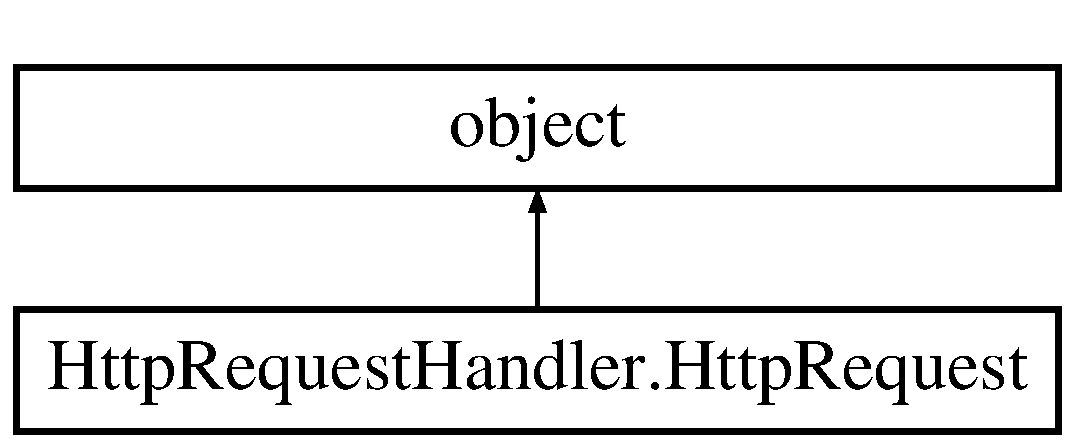
\includegraphics[height=2.000000cm]{class_http_request_handler_1_1_http_request}
\end{center}
\end{figure}
\subsection*{Public Member Functions}
\begin{DoxyCompactItemize}
\item 
\hypertarget{class_http_request_handler_1_1_http_request_a30bc663deb6096f298b2fef1a7ce9194}{def {\bfseries \-\_\-\-\_\-init\-\_\-\-\_\-}}\label{class_http_request_handler_1_1_http_request_a30bc663deb6096f298b2fef1a7ce9194}

\item 
\hypertarget{class_http_request_handler_1_1_http_request_ab9d518b2d0bd87a15f35e8a40fe2bdcc}{def {\bfseries dump}}\label{class_http_request_handler_1_1_http_request_ab9d518b2d0bd87a15f35e8a40fe2bdcc}

\end{DoxyCompactItemize}
\subsection*{Public Attributes}
\begin{DoxyCompactItemize}
\item 
\hypertarget{class_http_request_handler_1_1_http_request_afee3737b9f3aaa34093bd28d6a998757}{{\bfseries browser}}\label{class_http_request_handler_1_1_http_request_afee3737b9f3aaa34093bd28d6a998757}

\item 
\hypertarget{class_http_request_handler_1_1_http_request_a595d62f9aba63eb3f22c6105805a3c91}{{\bfseries content\-Encoding}}\label{class_http_request_handler_1_1_http_request_a595d62f9aba63eb3f22c6105805a3c91}

\item 
\hypertarget{class_http_request_handler_1_1_http_request_ad4edb498e810e126fcc43c3725180228}{{\bfseries content\-Length}}\label{class_http_request_handler_1_1_http_request_ad4edb498e810e126fcc43c3725180228}

\item 
\hypertarget{class_http_request_handler_1_1_http_request_ad0dd413ed4621f1b086478cd63aa1b7d}{{\bfseries content\-Type}}\label{class_http_request_handler_1_1_http_request_ad0dd413ed4621f1b086478cd63aa1b7d}

\item 
\hypertarget{class_http_request_handler_1_1_http_request_afa5970c2f157d45f60b3697f869fe27f}{{\bfseries cookies}}\label{class_http_request_handler_1_1_http_request_afa5970c2f157d45f60b3697f869fe27f}

\item 
\hypertarget{class_http_request_handler_1_1_http_request_a74dc51f5b7df6d77193d271fcf70d4ce}{{\bfseries form}}\label{class_http_request_handler_1_1_http_request_a74dc51f5b7df6d77193d271fcf70d4ce}

\item 
\hypertarget{class_http_request_handler_1_1_http_request_a8f88228ec44ba91ad375b239ec24216d}{{\bfseries headers}}\label{class_http_request_handler_1_1_http_request_a8f88228ec44ba91ad375b239ec24216d}

\item 
\hypertarget{class_http_request_handler_1_1_http_request_ab547a129480a5535290f9889ea8727b1}{{\bfseries method}}\label{class_http_request_handler_1_1_http_request_ab547a129480a5535290f9889ea8727b1}

\item 
\hypertarget{class_http_request_handler_1_1_http_request_a4c47318b09d00228ef9cdeeac36411d4}{{\bfseries query\-Strings}}\label{class_http_request_handler_1_1_http_request_a4c47318b09d00228ef9cdeeac36411d4}

\item 
\hypertarget{class_http_request_handler_1_1_http_request_aba42a32d838dae8eb146ee09a46df015}{{\bfseries referrer}}\label{class_http_request_handler_1_1_http_request_aba42a32d838dae8eb146ee09a46df015}

\item 
\hypertarget{class_http_request_handler_1_1_http_request_ae966be257b4bf488900e50244c9c685a}{{\bfseries user\-Agent}}\label{class_http_request_handler_1_1_http_request_ae966be257b4bf488900e50244c9c685a}

\item 
\hypertarget{class_http_request_handler_1_1_http_request_a6009e1c69c3865bbf50e81aa30dfff55}{{\bfseries user\-Host\-Address}}\label{class_http_request_handler_1_1_http_request_a6009e1c69c3865bbf50e81aa30dfff55}

\item 
\hypertarget{class_http_request_handler_1_1_http_request_abcfd7eff17c60a2037b9703f2ad94f33}{{\bfseries user\-Host\-Name}}\label{class_http_request_handler_1_1_http_request_abcfd7eff17c60a2037b9703f2ad94f33}

\item 
\hypertarget{class_http_request_handler_1_1_http_request_aefada851f3f8589e672abcce4631565a}{{\bfseries user\-Languages}}\label{class_http_request_handler_1_1_http_request_aefada851f3f8589e672abcce4631565a}

\item 
\hypertarget{class_http_request_handler_1_1_http_request_a83e7bf9c3f072cefebb6fe85d30baca2}{{\bfseries request\-Uri}}\label{class_http_request_handler_1_1_http_request_a83e7bf9c3f072cefebb6fe85d30baca2}

\item 
\hypertarget{class_http_request_handler_1_1_http_request_aa1a596471873ebb1bf6d63bd2f410bcc}{{\bfseries http\-Version}}\label{class_http_request_handler_1_1_http_request_aa1a596471873ebb1bf6d63bd2f410bcc}

\item 
\hypertarget{class_http_request_handler_1_1_http_request_a8e5e375e07703a121b490603b4695f28}{{\bfseries ready}}\label{class_http_request_handler_1_1_http_request_a8e5e375e07703a121b490603b4695f28}

\end{DoxyCompactItemize}
\subsection*{Static Public Attributes}
\begin{DoxyCompactItemize}
\item 
\hypertarget{class_http_request_handler_1_1_http_request_a950f8a27a420caf0382c2bf05b5b1cc3}{int {\bfseries M\-A\-X\-\_\-\-H\-E\-A\-D\-E\-R\-\_\-\-L\-E\-N\-G\-T\-H} = 8}\label{class_http_request_handler_1_1_http_request_a950f8a27a420caf0382c2bf05b5b1cc3}

\end{DoxyCompactItemize}


The documentation for this class was generated from the following file\-:\begin{DoxyCompactItemize}
\item 
/home/ivan/\-Code\-Snippets-\/\-Projects/\-Telebid-\/\-Tasks/\-Web\-Server/\-Async\-Server/Http\-Request\-Handler.\-py\end{DoxyCompactItemize}

\hypertarget{class_http_request_handler_1_1_http_request_handler}{\section{Http\-Request\-Handler.\-Http\-Request\-Handler Class Reference}
\label{class_http_request_handler_1_1_http_request_handler}\index{Http\-Request\-Handler.\-Http\-Request\-Handler@{Http\-Request\-Handler.\-Http\-Request\-Handler}}
}
Inheritance diagram for Http\-Request\-Handler.\-Http\-Request\-Handler\-:\begin{figure}[H]
\begin{center}
\leavevmode
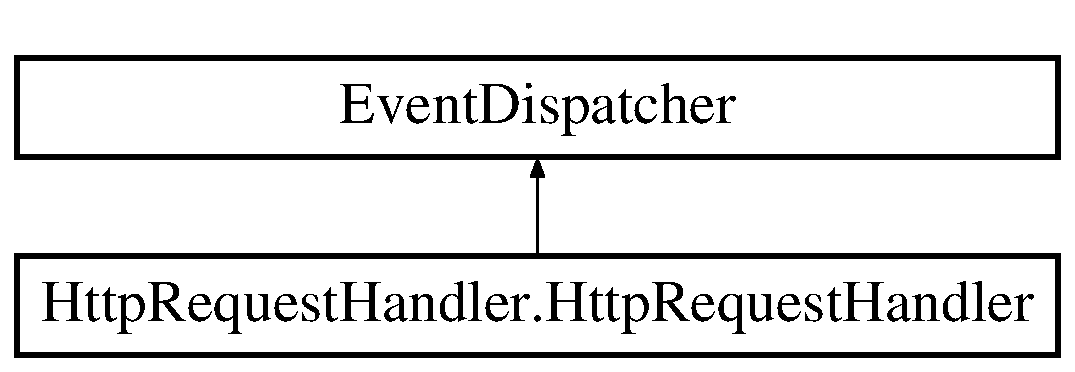
\includegraphics[height=2.000000cm]{class_http_request_handler_1_1_http_request_handler}
\end{center}
\end{figure}
\subsection*{Public Member Functions}
\begin{DoxyCompactItemize}
\item 
\hypertarget{class_http_request_handler_1_1_http_request_handler_a4954fb9400047a85dc5475f292159ed4}{def {\bfseries \-\_\-\-\_\-init\-\_\-\-\_\-}}\label{class_http_request_handler_1_1_http_request_handler_a4954fb9400047a85dc5475f292159ed4}

\item 
\hypertarget{class_http_request_handler_1_1_http_request_handler_a02f0499dbbcb23259ddb69e5be9d4989}{def {\bfseries handle\-\_\-event}}\label{class_http_request_handler_1_1_http_request_handler_a02f0499dbbcb23259ddb69e5be9d4989}

\end{DoxyCompactItemize}
\subsection*{Public Attributes}
\begin{DoxyCompactItemize}
\item 
\hypertarget{class_http_request_handler_1_1_http_request_handler_a47d6f6ab71f8b3134ef847b26aecc55c}{{\bfseries connection}}\label{class_http_request_handler_1_1_http_request_handler_a47d6f6ab71f8b3134ef847b26aecc55c}

\item 
\hypertarget{class_http_request_handler_1_1_http_request_handler_aee0a4b43025c870322a68ffd57d45dd0}{{\bfseries state}}\label{class_http_request_handler_1_1_http_request_handler_aee0a4b43025c870322a68ffd57d45dd0}

\item 
\hypertarget{class_http_request_handler_1_1_http_request_handler_a2694e1a5ce08a8de444f94eb8c70687c}{{\bfseries current\-\_\-request}}\label{class_http_request_handler_1_1_http_request_handler_a2694e1a5ce08a8de444f94eb8c70687c}

\item 
\hypertarget{class_http_request_handler_1_1_http_request_handler_a2e09a168e2824fb6cedb8b29702ba88b}{{\bfseries task\-\_\-manager}}\label{class_http_request_handler_1_1_http_request_handler_a2e09a168e2824fb6cedb8b29702ba88b}

\item 
\hypertarget{class_http_request_handler_1_1_http_request_handler_a23222cba655432a8dbb77997686bb372}{{\bfseries request\-\_\-queue}}\label{class_http_request_handler_1_1_http_request_handler_a23222cba655432a8dbb77997686bb372}

\item 
\hypertarget{class_http_request_handler_1_1_http_request_handler_ac14cba087cc7bb12f60c4cb272f83fba}{{\bfseries processing}}\label{class_http_request_handler_1_1_http_request_handler_ac14cba087cc7bb12f60c4cb272f83fba}

\end{DoxyCompactItemize}
\subsection*{Static Public Attributes}
\begin{DoxyCompactItemize}
\item 
\hypertarget{class_http_request_handler_1_1_http_request_handler_a60ad60b9b4b74a703ffeae8fb72fd9ca}{tuple {\bfseries find\-\_\-request\-\_\-line} = re.\-compile(b\char`\"{}($^\wedge$G\-E\-T)\textbackslash{}s(.$\ast$)(?=\textbackslash{}s\-H\-T\-T\-P)(\textbackslash{}s\-H\-T\-T\-P\textbackslash{}/)(\mbox{[}1\mbox{]}\textbackslash{}.\mbox{[}0-\/1\mbox{]})\char`\"{})}\label{class_http_request_handler_1_1_http_request_handler_a60ad60b9b4b74a703ffeae8fb72fd9ca}

\item 
\hypertarget{class_http_request_handler_1_1_http_request_handler_a550d250b1266add5a833b70137bb359d}{tuple {\bfseries find\-\_\-headers} = re.\-compile(b\char`\"{}(.$\ast$)\-:\textbackslash{}s(.$\ast$)\char`\"{})}\label{class_http_request_handler_1_1_http_request_handler_a550d250b1266add5a833b70137bb359d}

\end{DoxyCompactItemize}


The documentation for this class was generated from the following file\-:\begin{DoxyCompactItemize}
\item 
/home/ivan/\-Code\-Snippets-\/\-Projects/\-Telebid-\/\-Tasks/\-Web\-Server/\-Async\-Server/Http\-Request\-Handler.\-py\end{DoxyCompactItemize}

\hypertarget{class_http_response_1_1_http_response}{\section{Http\-Response.\-Http\-Response Class Reference}
\label{class_http_response_1_1_http_response}\index{Http\-Response.\-Http\-Response@{Http\-Response.\-Http\-Response}}
}
Inheritance diagram for Http\-Response.\-Http\-Response\-:\begin{figure}[H]
\begin{center}
\leavevmode
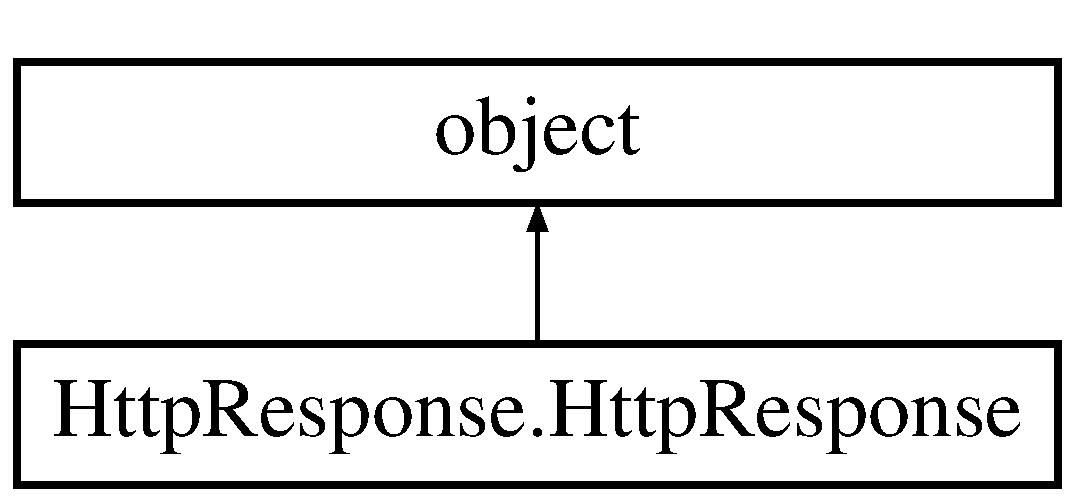
\includegraphics[height=2.000000cm]{class_http_response_1_1_http_response}
\end{center}
\end{figure}
\subsection*{Public Member Functions}
\begin{DoxyCompactItemize}
\item 
\hypertarget{class_http_response_1_1_http_response_a70270df83b9b93669fb29bb06d6b39dc}{def {\bfseries \-\_\-\-\_\-init\-\_\-\-\_\-}}\label{class_http_response_1_1_http_response_a70270df83b9b93669fb29bb06d6b39dc}

\item 
\hypertarget{class_http_response_1_1_http_response_a100e9b3df1551b7934d83c24ea7c5d0f}{def {\bfseries generate}}\label{class_http_response_1_1_http_response_a100e9b3df1551b7934d83c24ea7c5d0f}

\item 
\hypertarget{class_http_response_1_1_http_response_a340c587e2e3e509d57b2e2adb51aeebf}{def {\bfseries raw}}\label{class_http_response_1_1_http_response_a340c587e2e3e509d57b2e2adb51aeebf}

\end{DoxyCompactItemize}
\subsection*{Public Attributes}
\begin{DoxyCompactItemize}
\item 
\hypertarget{class_http_response_1_1_http_response_acbd04b682c461462dee12e974f087499}{{\bfseries http\-Version}}\label{class_http_response_1_1_http_response_acbd04b682c461462dee12e974f087499}

\item 
\hypertarget{class_http_response_1_1_http_response_af640be8844ce87ab7ed222ed8da6f6f1}{{\bfseries status\-Code}}\label{class_http_response_1_1_http_response_af640be8844ce87ab7ed222ed8da6f6f1}

\item 
\hypertarget{class_http_response_1_1_http_response_a772463ab8041c405927818926bdb4370}{{\bfseries reason\-Phase}}\label{class_http_response_1_1_http_response_a772463ab8041c405927818926bdb4370}

\item 
\hypertarget{class_http_response_1_1_http_response_a3d7a11cb3f47a0d21ab9b6814da0828c}{{\bfseries headers}}\label{class_http_response_1_1_http_response_a3d7a11cb3f47a0d21ab9b6814da0828c}

\end{DoxyCompactItemize}


The documentation for this class was generated from the following file\-:\begin{DoxyCompactItemize}
\item 
/home/ivan/\-Code\-Snippets-\/\-Projects/\-Telebid-\/\-Tasks/\-Web\-Server/\-Async\-Server/Http\-Response.\-py\end{DoxyCompactItemize}

\hypertarget{class_task_manager_1_1_task}{\section{Task\-Manager.\-Task Class Reference}
\label{class_task_manager_1_1_task}\index{Task\-Manager.\-Task@{Task\-Manager.\-Task}}
}
Inheritance diagram for Task\-Manager.\-Task\-:\begin{figure}[H]
\begin{center}
\leavevmode
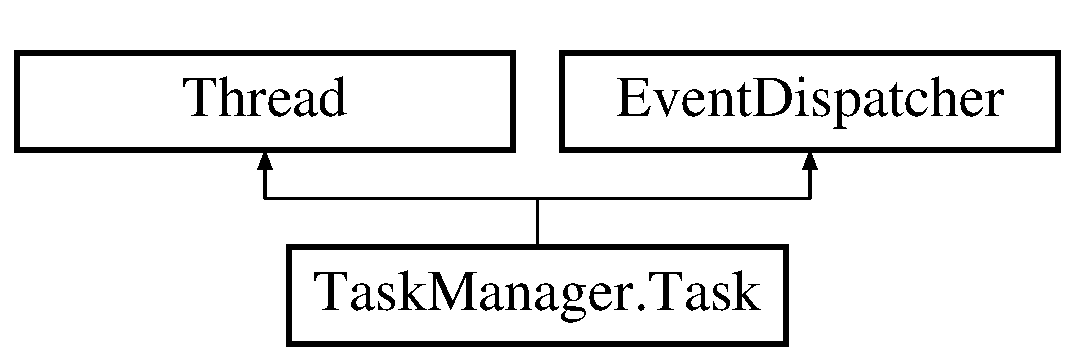
\includegraphics[height=2.000000cm]{class_task_manager_1_1_task}
\end{center}
\end{figure}
\subsection*{Public Member Functions}
\begin{DoxyCompactItemize}
\item 
\hypertarget{class_task_manager_1_1_task_a90b356b61e49c026c99d5814538c534a}{def {\bfseries \-\_\-\-\_\-init\-\_\-\-\_\-}}\label{class_task_manager_1_1_task_a90b356b61e49c026c99d5814538c534a}

\item 
\hypertarget{class_task_manager_1_1_task_a163d160cf661a7ec691a5c0fadbfe942}{def {\bfseries run}}\label{class_task_manager_1_1_task_a163d160cf661a7ec691a5c0fadbfe942}

\end{DoxyCompactItemize}
\subsection*{Public Attributes}
\begin{DoxyCompactItemize}
\item 
\hypertarget{class_task_manager_1_1_task_aaf5bc8de56df591ae91f7970a0890759}{{\bfseries file}}\label{class_task_manager_1_1_task_aaf5bc8de56df591ae91f7970a0890759}

\item 
\hypertarget{class_task_manager_1_1_task_aa5da638c40484b20cac2ebf1a5b925d7}{{\bfseries type}}\label{class_task_manager_1_1_task_aa5da638c40484b20cac2ebf1a5b925d7}

\item 
\hypertarget{class_task_manager_1_1_task_a3a0a2cdf2a9074e42db218abaa0c4733}{{\bfseries file\-\_\-path}}\label{class_task_manager_1_1_task_a3a0a2cdf2a9074e42db218abaa0c4733}

\item 
\hypertarget{class_task_manager_1_1_task_a69c6b2475d8073b93b030cc0203a22dc}{{\bfseries done}}\label{class_task_manager_1_1_task_a69c6b2475d8073b93b030cc0203a22dc}

\end{DoxyCompactItemize}


The documentation for this class was generated from the following file\-:\begin{DoxyCompactItemize}
\item 
/home/ivan/\-Code\-Snippets-\/\-Projects/\-Telebid-\/\-Tasks/\-Web\-Server/\-Async\-Server/Task\-Manager.\-py\end{DoxyCompactItemize}

\hypertarget{class_task_manager_1_1_task_manager}{\section{Task\-Manager.\-Task\-Manager Class Reference}
\label{class_task_manager_1_1_task_manager}\index{Task\-Manager.\-Task\-Manager@{Task\-Manager.\-Task\-Manager}}
}
Inheritance diagram for Task\-Manager.\-Task\-Manager\-:\begin{figure}[H]
\begin{center}
\leavevmode
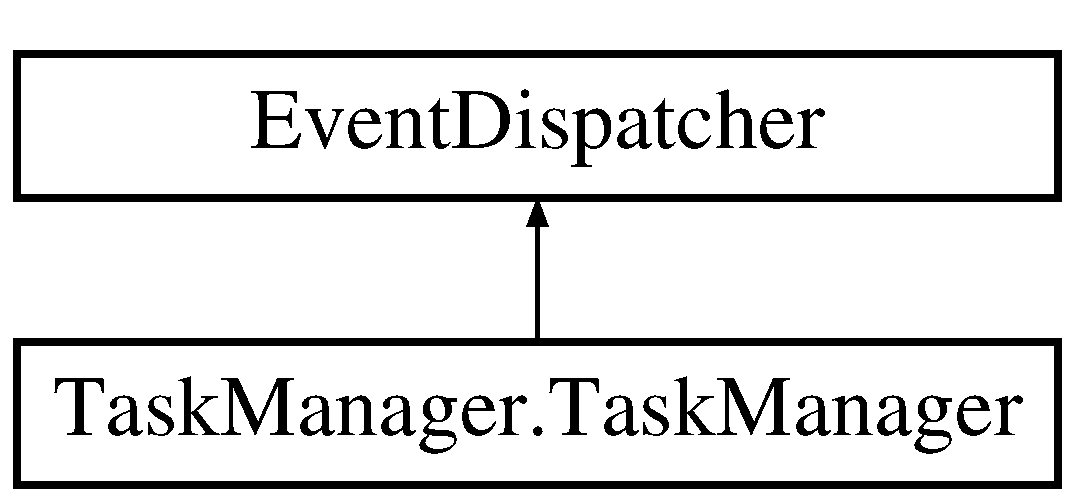
\includegraphics[height=2.000000cm]{class_task_manager_1_1_task_manager}
\end{center}
\end{figure}
\subsection*{Public Member Functions}
\begin{DoxyCompactItemize}
\item 
\hypertarget{class_task_manager_1_1_task_manager_aa82c3de5047eaa601901d9bba3c0b347}{def {\bfseries \-\_\-\-\_\-init\-\_\-\-\_\-}}\label{class_task_manager_1_1_task_manager_aa82c3de5047eaa601901d9bba3c0b347}

\item 
\hypertarget{class_task_manager_1_1_task_manager_a630d6f3fda9e0acc504e65236f923fa9}{def {\bfseries handle\-\_\-event}}\label{class_task_manager_1_1_task_manager_a630d6f3fda9e0acc504e65236f923fa9}

\end{DoxyCompactItemize}
\subsection*{Public Attributes}
\begin{DoxyCompactItemize}
\item 
\hypertarget{class_task_manager_1_1_task_manager_a87766832accfef894e63b6510d113817}{{\bfseries tasks}}\label{class_task_manager_1_1_task_manager_a87766832accfef894e63b6510d113817}

\end{DoxyCompactItemize}


The documentation for this class was generated from the following file\-:\begin{DoxyCompactItemize}
\item 
/home/ivan/\-Code\-Snippets-\/\-Projects/\-Telebid-\/\-Tasks/\-Web\-Server/\-Async\-Server/Task\-Manager.\-py\end{DoxyCompactItemize}

%--- End generated contents ---

% Index
\newpage
\phantomsection
\addcontentsline{toc}{chapter}{Index}
\printindex

\end{document}
